%% LyX 2.3.4.2 created this file.  For more info, see http://www.lyx.org/.
%% Do not edit unless you really know what you are doing.
\documentclass[english]{article}
\usepackage[T1]{fontenc}
\usepackage[latin9]{inputenc}
\usepackage{verbatim}
\usepackage{float}
\usepackage{graphicx}

\makeatletter

%%%%%%%%%%%%%%%%%%%%%%%%%%%%%% LyX specific LaTeX commands.
%% A simple dot to overcome graphicx limitations
\newcommand{\lyxdot}{.}


\makeatother

\usepackage{babel}
\begin{document}
\title{Prediction of Protein-Protein Interactions on the Human and Rice Interactome }
\author{Nicol�s Antonio L�pez Rozo}
\maketitle
\begin{abstract}

Past work on applying network analyses to predict unmapped protein-protein interactions
(PPI) suggests that the higher the number of paths of length\textasciitilde 3
(L3) between two proteins, the more likely they are to interact. This
paper extends previous results based on the L3 principle by taking into
account the representation learning of node features of the PPI network.
In particular, the proposed \texttt{XGBoost} model uses L3 and other handcrafted
features, as well learned features from \texttt{Node2Vec} embeddings. Our main result
shows that while L3 is an important feature for predicting links,
better performance is achieved when the measure is combined with edge embeddings. Our approach is evaluated for the human and rice interactomes.
\end{abstract}
\begin{comment}
need include a feature that compares the dimension of the embedding
is useful for prediction with L3 to show that they independent measures
- we do not want to be learning L3 through node2vec
\end{comment}


\section{Introduction}

\begin{comment}
Need to add other relevant references
\end{comment}

Proteins are key actors of biological processes inside cells.
They function as are part of dynamic networks of protein-protein
interactions (PPI) rather than carrying out a variety of tasks as isolated
agents~\cite{Lin2017}. At the cellular level, PPI networks play a key role in
a number of interdependent mechanisms, including signal transduction,
homeostasis control, stress responses, plant defense and organ formation.
At the molecular level, PPI networks also play an essential role in physiological
and developmental processes, including protein phosphorylation, transcriptional
co-factor recruitment and transporter activation~\cite{Zhang_2010_PPI}.

%Prediction of potentially relevant yet unexplored PPIs is a current research topic on bioinformatics. 
Several authors have introduced different
methods for extrapolating information from PPI networks.
Kovacs et al. (2019) proposes an approach which relies on counting
paths of length 3 (L3) to predict interactions among proteins for
a variety of model organisms. The proposed approach outperforms previous
methods for PPI networks of yeast (\emph{S. cerevisiae}),
Arabidopsis (\emph{A. thaliana}), worm (\emph{C. elegans}), fly (\emph{D.
melanogaster}), fission yeast (\emph{S. pombe}) and mouse (\emph{M.
musculus}), as well as for the human interactome \cite{Kovacs2019}.

A common way to uncover (or validate) PPIs is the \emph{yeast-two-hybrid} or \emph{Y2H}
technique (also known as \emph{two-hybrid screening}). Y2H is based on the expression of a so called reporter gene that is
activated by the binding of a DNA-binding domain and an activation
domain of a transcription factor. This transcription factor then binds to an upstream activation
sequence. For the Y2H technique, a protein is fused to the DNA-binding domain (known as \emph{bait}) and another protein to the activation domain (known as
\emph{prey}). Only when the proteins interact, the reporter gene
is expressed. Otherwise, the reporter gene expression is activated
by the activation domain.

\begin{comment}
NL: I will make this figure myself

JF: Good idea
\end{comment}

\begin{figure}[h]
\caption{Yeast-2-Hybrid Technique}

\noindent \centering{}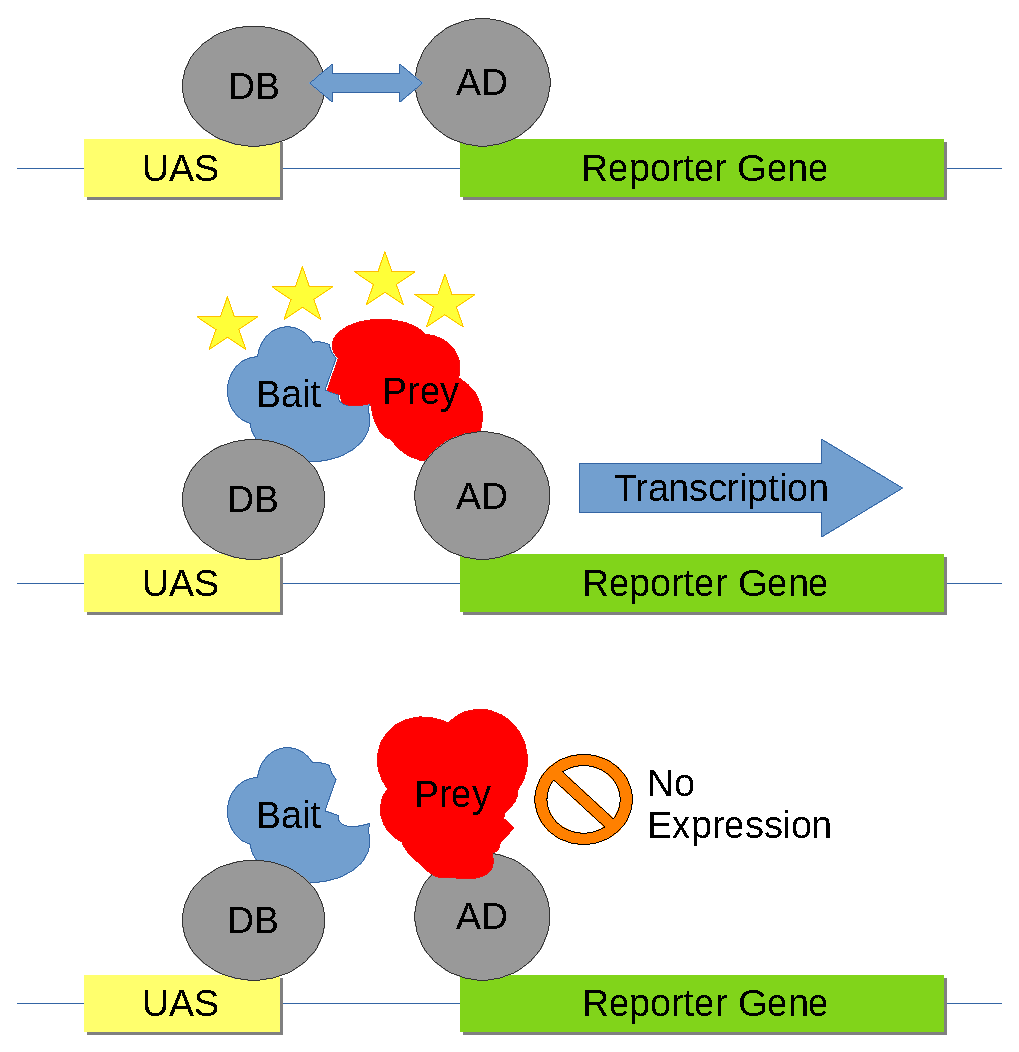
\includegraphics[width=1\columnwidth]{Y2H}
\end{figure}

PPI networks are constructed based on the outcome of numerous Y2H experiments in which known interactions for each protein are represented. 
Several algorithms are proposed over these networks in order to predict
hidden interactions. This paper evaluates PPI predictions based on
three measures: the count of paths of length 2 or Common Neighbors (\textbf{CN}); the raw count of paths of length 3 (\textbf{A3}); and the degree-normalized count of paths of length 3 (\textbf{L3}).

%Furthermore

\begin{comment}
JF: Yet you do more than evaluating this three measures so this has
to be updated.

JF: Not sure we should use L3 above since it is being redefined as
a normalized measure here!
\end{comment}

Our focus is to evaluate different methods for predicting
PPIs using the existing knowledge of the network of interactions,
which is represented as an undirected graph. 
\begin{comment}
    not sure we can call the TCP approach the traditional approach
\end{comment}

% The traditional way of approaching the problem is usually based on social networks analysis,
% more specifically on the triadic closure principle (TCP), that states
% that the more common shared friends that two people have, the more
% likely that they know each other. As shown by previous studies, the
% mentioned approach fails because it does not consider the structural
% and chemical properties of the proteins \cite{Kovacs2019}.

Human and rice PPI networks are used to compare state-of-the-art methods
%what are these state of the art methods?
, as well as the proposed approach (CN, A3, L3). In the case of the human network, the human interactome dataset denoted by \emph{HI-II-14} and its curated version (\emph{HI-TESTED})
were used for evaluation. Results on experimental assays are consolidated to build a validation network denoted by \emph{HI-III}. 

\begin{comment}
JF: need to comment on rice as well  (in the same section). Or move the discussion above to Material and Methods

JF: read throughout the document but edited up here. I prefer to read
the results before editing the materials and methods section. 
\end{comment}


\section{Materials and Methods}

\subsection{Data Availability}

Human interactome data and base source code were downloaded from the
repository of the length-3 degree normalized paths methodology \cite{Kovacs2019}:
the datasets \emph{HI-II-14} and \emph{HI-TESTED} are used for prediction
and the dataset \emph{HI-III} is used for validation.

\begin{comment}
    JF: I thought you were generating \emph{HI-III} based on your results - this is confusing
    
    \end{comment}

Rice interactome information was downloaded from the STRING database
\cite{Szklarczyk2019}, corresponding to the \emph{Oryza sativa} subspecies.
The file labelled \emph{4530.protein.links.detailed.v11.0.txt}.
contains more than 8 million PPIs from several sources. For
the purpose of this study, only PPIs with
evidence from curated databases are considered (i.e. rows where the column
\emph{databases} has a value greater than zero). The resulting network consists of
$5025$ nodes and $164420$ edges.

\subsection{Code Implementation}

Previous code implementation was adapted from \texttt{C++} to \texttt{Python}
(V3.6), in order to unify the algorithms into one single script. 
% from the perspective of the reader what other code was in Python?
For
the purpose of algorithmic validation, the three methods were implemented
from scratch with basic functionalities and data structures of the
\texttt{Python} language.

\subsection{Data Preprocessing}

Information for the human interactome was used as-is, which corresponds
to networks of $4298$, $3727$ and $5604$ proteins and $13868$,
$9433$ and $23322$ interactions, respectively.

For the rice interactome, an additional preprocessing was performed.
The filtered network for rice consists of $5025$ proteins (nodes)
and $164420$ interactions (edges) distributed among $178$ connected
components. The connected component with the greatest number of edges
was selected in this case. The extracted connected component consists
of $n=4390$ nodes and $m=163319$ edges, which corresponds to $99.33%\%
$ of filtered edges. Further investigation is applied to this network,
which is very similar in number of nodes to the curated information
on the human interactome, although rice network is much more connected.

\subsection{Edge Prediction}

For the interaction prediction for each network, the algorithms described
below were used. It is important to keep in mind how the protein-protein
interaction (PPI) network $G=(V,E)$ is conceptualized: each node
($v_{i}\in V$) represents a protein and each undirected edge ($e_{b}=\{v_{i},v_{j}\},\,e_{b}\in E$)
represents and interaction among proteins $v_{i}$ and $v_{j}$.
\begin{description}
\item [{Common~Neighbors~(CN)}] This method is based on the Triadic Closure
Principle: ``the more common friends two individuals have, the more
likely that they know each other''. For the implementation of this
method, $A{{}^2}$ matrix is calculated, being $A$ the adjacency
matrix of the network.
\item [{Length-3~Paths~(A3)}] This is the simplest implementation of
the proposed insight of ``if my friends and your friends interact,
then we might interact too''. The calculating is carried on with
$A{{}^3}$, i.e, the third power of the adjacency matrix.
\item [{Degree-normalized~L-3~Score~(L3)}] The previous approach might
overestimate the importance of some edges due to intermediate hubs
which add many shortcuts in the graph. To address that issue, a degree
normalization for the path $X\rightarrow U\rightarrow V\rightarrow Y$
is applied by considering the degree $k$ of the intermediate nodes
$U$ and $V$, as follows.
\[
p_{XY}=\sum_{U,V}\frac{A_{XU}\cdot A_{UV}\cdot A_{VY}}{\sqrt{k_{U}\cdot k_{V}}}
\]
\\
where $A_{ij}$ represents the value of the adjacency matrix for nodes
$i$ and $j$: 1 if the edge $\{i,j\}$ exists, 0 otherwise.
\end{description}

\subsection{Sampling Procedure}

For each network of protein interactions, the following procedure
was performed 10 times in order to address the stochastic nature of
the process and have a consensus:
\begin{itemize}
\item A percentage of interactions is removed at random from the network
(20\%).
\item The same amount of removed interactions are then predicted using the
main methods for prediction mentioned by Kovacs et al (2019): Common
Neighbors (\textbf{A2}), raw path count of paths of length 3 (\textbf{A3})
and the Length-3 degree-normalized score (\textbf{L3}).
\item A test dataset is created as follows: all removed edges are included
(as observed positives for the ML algorithm) and from the predicted
edges of \textbf{A2}, \textbf{A3} and \textbf{L3} that don't lie in
the previous classification (observed negatives), a random subset
is chosen such that the dataset is balanced, that is, the amount of
observed positive labels is equal to the observed negative labels.
\item Once the dataset is ready, it is randomly partitioned: 80\% is used
for \texttt{XGBoost} model training and 20\% is used for validation.
It is important to have in mind that balanced distribution of the
positive and negative labels in the datasets was satisfied.
\end{itemize}
It is worth mentioning that some exploration experiments were carried
out with interactions removal percentages of 2, 5, 10 and 20\%, as
well as train-test partitions of 15-85, 80-20 and 75-25, and the explained
parameter set was selected because it either represented a marginal
gain (results not shown) or because it was a common parameter selection
in related literature.

\subsection{Feature Extraction with \texttt{Node2Vec}}

The \texttt{Node2Vec} module was used for extracting features of the
rice interactome graph. The parameters and considerations for the
model were:
\begin{itemize}
\item All paths in the random walks are equally likely (\texttt{p=1, q=1})
\item Use a modest number of dimensions and threads for calculation (\texttt{dimensions=16,
workers=4})
\item Since length-3 paths are the defining property in this study, there
is no necessity for longer walks. However, it is important to try
out many possible redundant routes and to consider a window of at
least 4 (\texttt{walk\_length=5, num\_walks=300, window=5})
\item Other standard parameters were left with default values (\texttt{min\_count=1,
batch\_words=4})
\item Edge embeddings were calculated using a geometric ratio of the node
embeddings (\texttt{HadamardEmbedder})
\end{itemize}

\subsection{Handcrafted Feature}

Due to the poor results of the \emph{raw} Length-3 counting (\textbf{A3}),
a different approach for this information was carried out in the present
study: As it still gives a lot of information that might be useful
for a predictive routine, this counting was normalized (dividing by
the greatest counting in the \textbf{A3} top predictions) and then
used as a feature for the Machine Learning algorithm. For completeness,
also \textbf{CN} and \textbf{L3} information was used as a possible
feature. Finally, the case were no handcrafted feature was also considered,
that is, only the features extracted from the structure of the network.

\subsection{Feature to Predict: Existence}

The feature to predict corresponds to the possible existence (\emph{True/False})
of a link based on the existing information of the network, using
the network itself in a random sub\_exploration (\texttt{Node2Vec})
as well as in a structured search (A3). This property is evaluated
by taking out a fraction of the edges and then trying to predict for
a given set of possible edges if they have a high probability to belong
to the original network.

\subsection{Machine Learning Algorithm}

The Extreme Gradient Boosting implementation of gradient boosted trees
is applied in this study to evaluate the existence of an edge. Gradient
boosted trees are usually used for supervised learning problems, where
the training data $X_{i}$ has multiple features and pretends to explain
(or predict) a target variable $Y_{i}$. The corresponding implementation
applied for this study is \texttt{XGBoost}, available publicly.

The selected parameters for the model were:\texttt{ max\_depth=3},
\texttt{colsample\_bytree=0.6} and \texttt{eval\_metric=''auc''}.

\subsection{Result Validation}

As mentioned before, 80\% of the final dataset was randomly selected
and used for training, while the remaining 20\% was used for validation.
The whole training-validation procedure was applied 10 times.

The chosen metric for validation was the Area under the Curve (\textbf{AUC})
of the Receiver Operating Characteristic (\textbf{ROC}). This curve
corresponds to plot the sensitivity (probability of predicting a real
positive as positive) against 1-specificity (probability of predicting
a real negative as positive). It is worth to remind that AUC values
move in the range $[0,1]$, where 1 is a perfect prediction and 0.5
corresponds to a random guess. Normally, values over 0.8 of AUC are
considered good.

\section{Results and Discussion}

\subsection{Rice Interactome}

For the rice interactome, the different model-features combinations
were trained and validated. After executing the mentioned routines,
the results are shown in Figure \ref{F1}. First, one should have
a baseline of comparison, which in this case corresponds to \texttt{Node2Vec}
without any additional feature included. The plot below shows those
results, and one can see that its mean performance using the AUC metric
is $0.52$, and that the results among the 10 repetitions are consistent.
This results mean that the model using only the default features perform
barely as good as a random choice of the labels. This result can also
be assessed when looking at the confusion matrix, where a precision
of $0.5168$ and a recall of $0.4589$ can be derived.

\begin{figure}[H]
\noindent \begin{centering}
\caption{\label{F1}Summary ROC curves for \texttt{Node2Vec} model alone}
\par\end{centering}
\noindent \raggedleft{}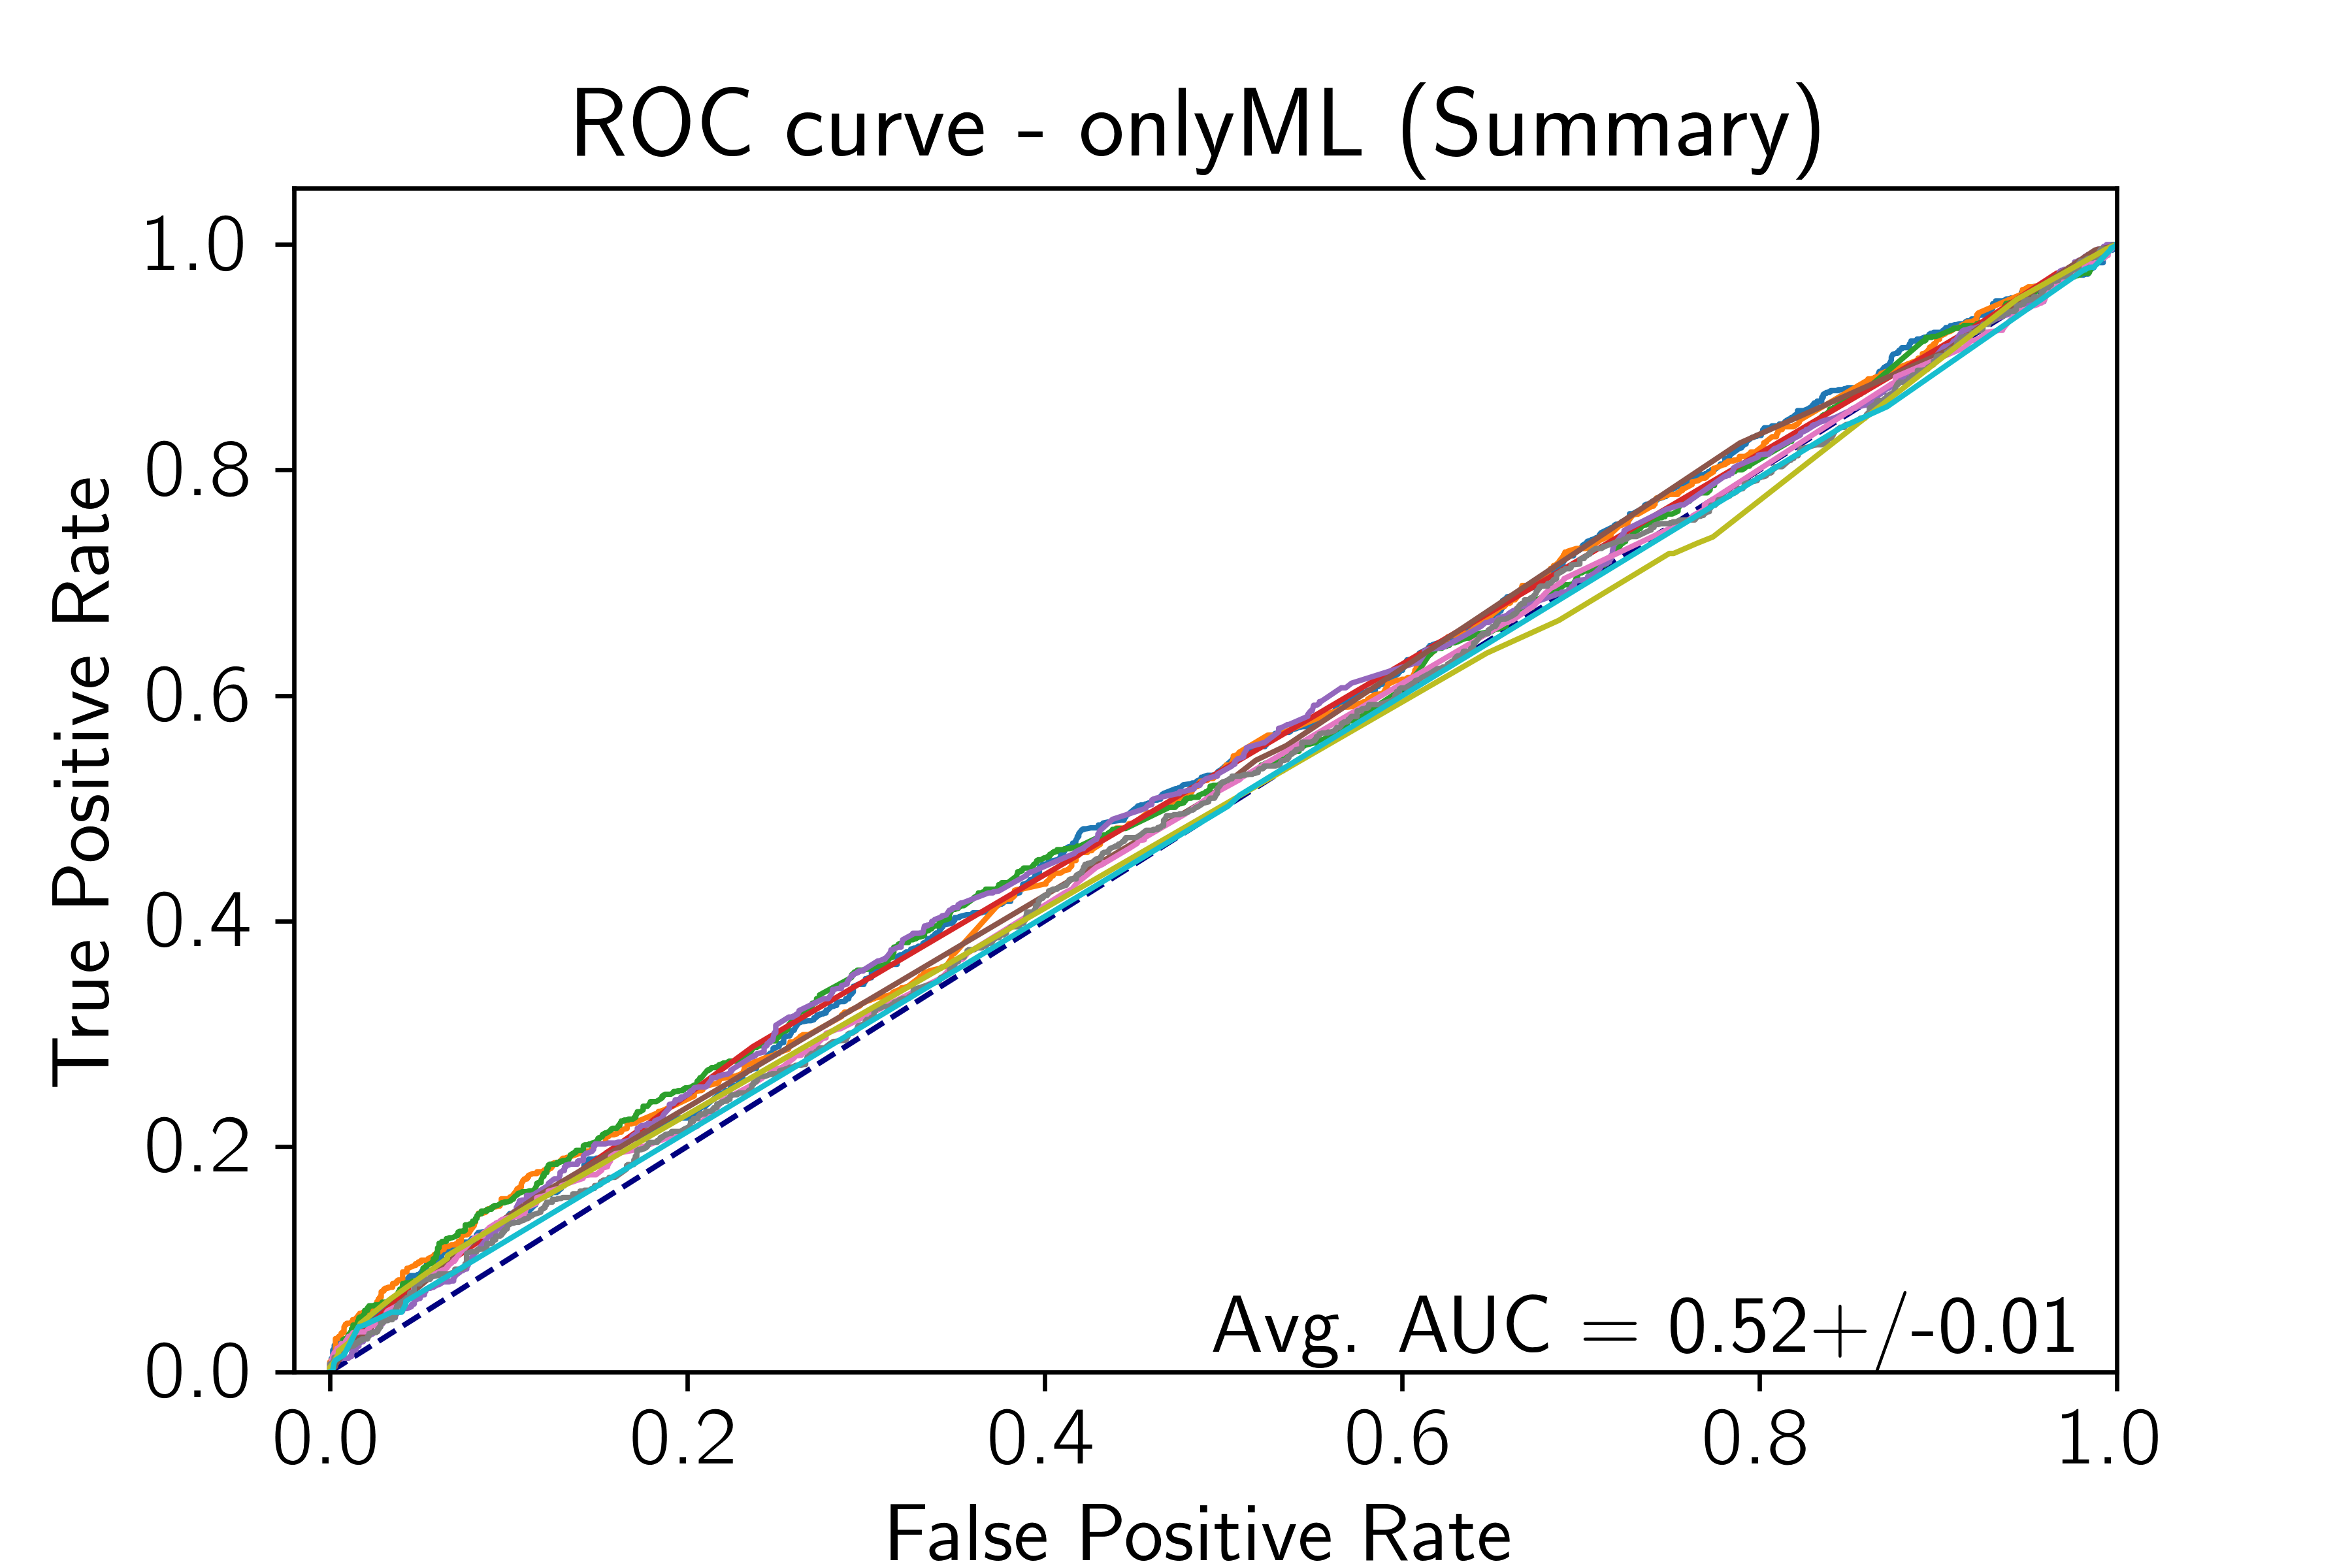
\includegraphics[width=0.48\columnwidth]{Only_ML/ROConlyML_SUMMARY}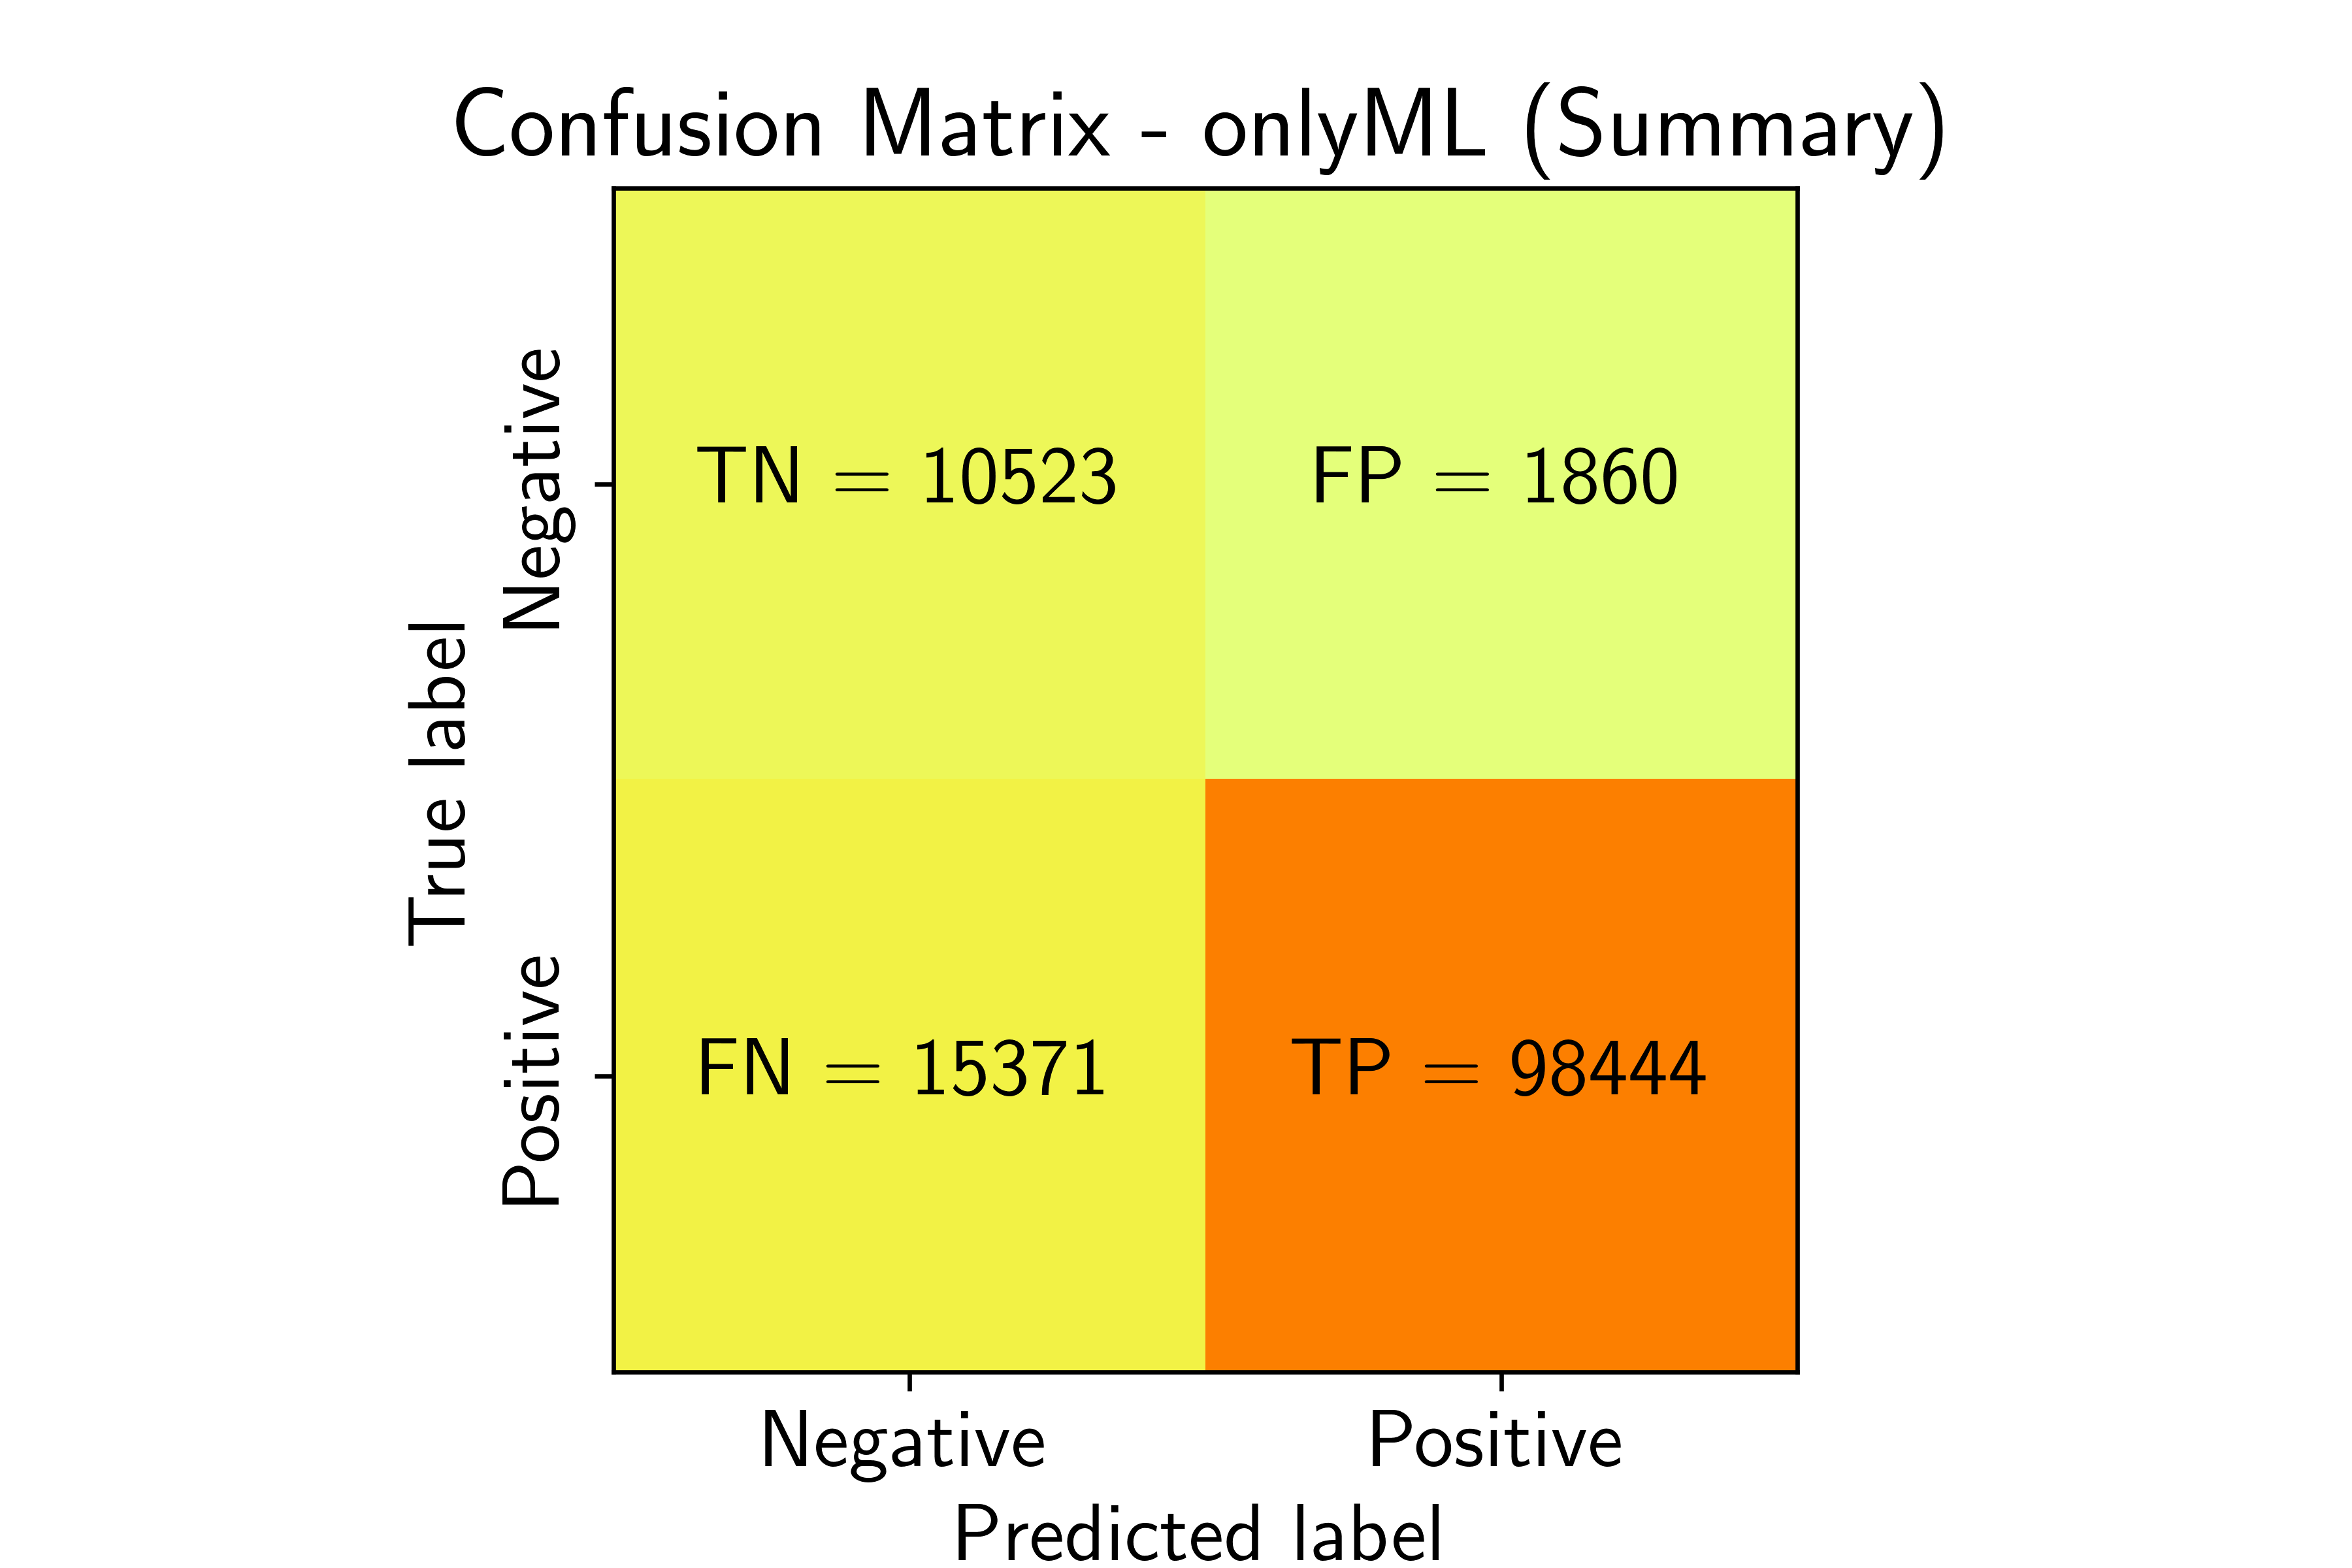
\includegraphics[width=0.48\columnwidth]{Only_ML/CMonlyML_SUMMARY}
\end{figure}

Next experiment carried out was to add each prediction method score
as a prediction feature, that is, use the score as the eleventh input
feature for the ML algorithm. Results for the Common Neighbors method
(\textbf{CN}), which uses paths of length 2, are shown in Figure \ref{F2}.
It can be observed again that all 10 experiments have small variability
among them and perform significantly better than the baseline, with
an area under the ROC curve of $0.90$, with small standard deviation.
When looking at the confusion matrix for this model, turns out that
most of the guesses are true positives and true negatives, resulting
in a precision of $0.93$ and a recall of $0.74$. Same analyses
are done with the count of paths of length 3 (\textbf{A3}) and with
the degree-normalized length-3 score (\textbf{L3}) and results are
presented in figures \ref{F3} and \ref{F4}, respectively, resulting
also in area under the curve of 0.9 for both cases.

\begin{figure}[H]
\noindent \begin{centering}
\caption{\label{F2}Results for \texttt{Node2Vec} model with CN feature}
\par\end{centering}
\noindent \raggedleft{}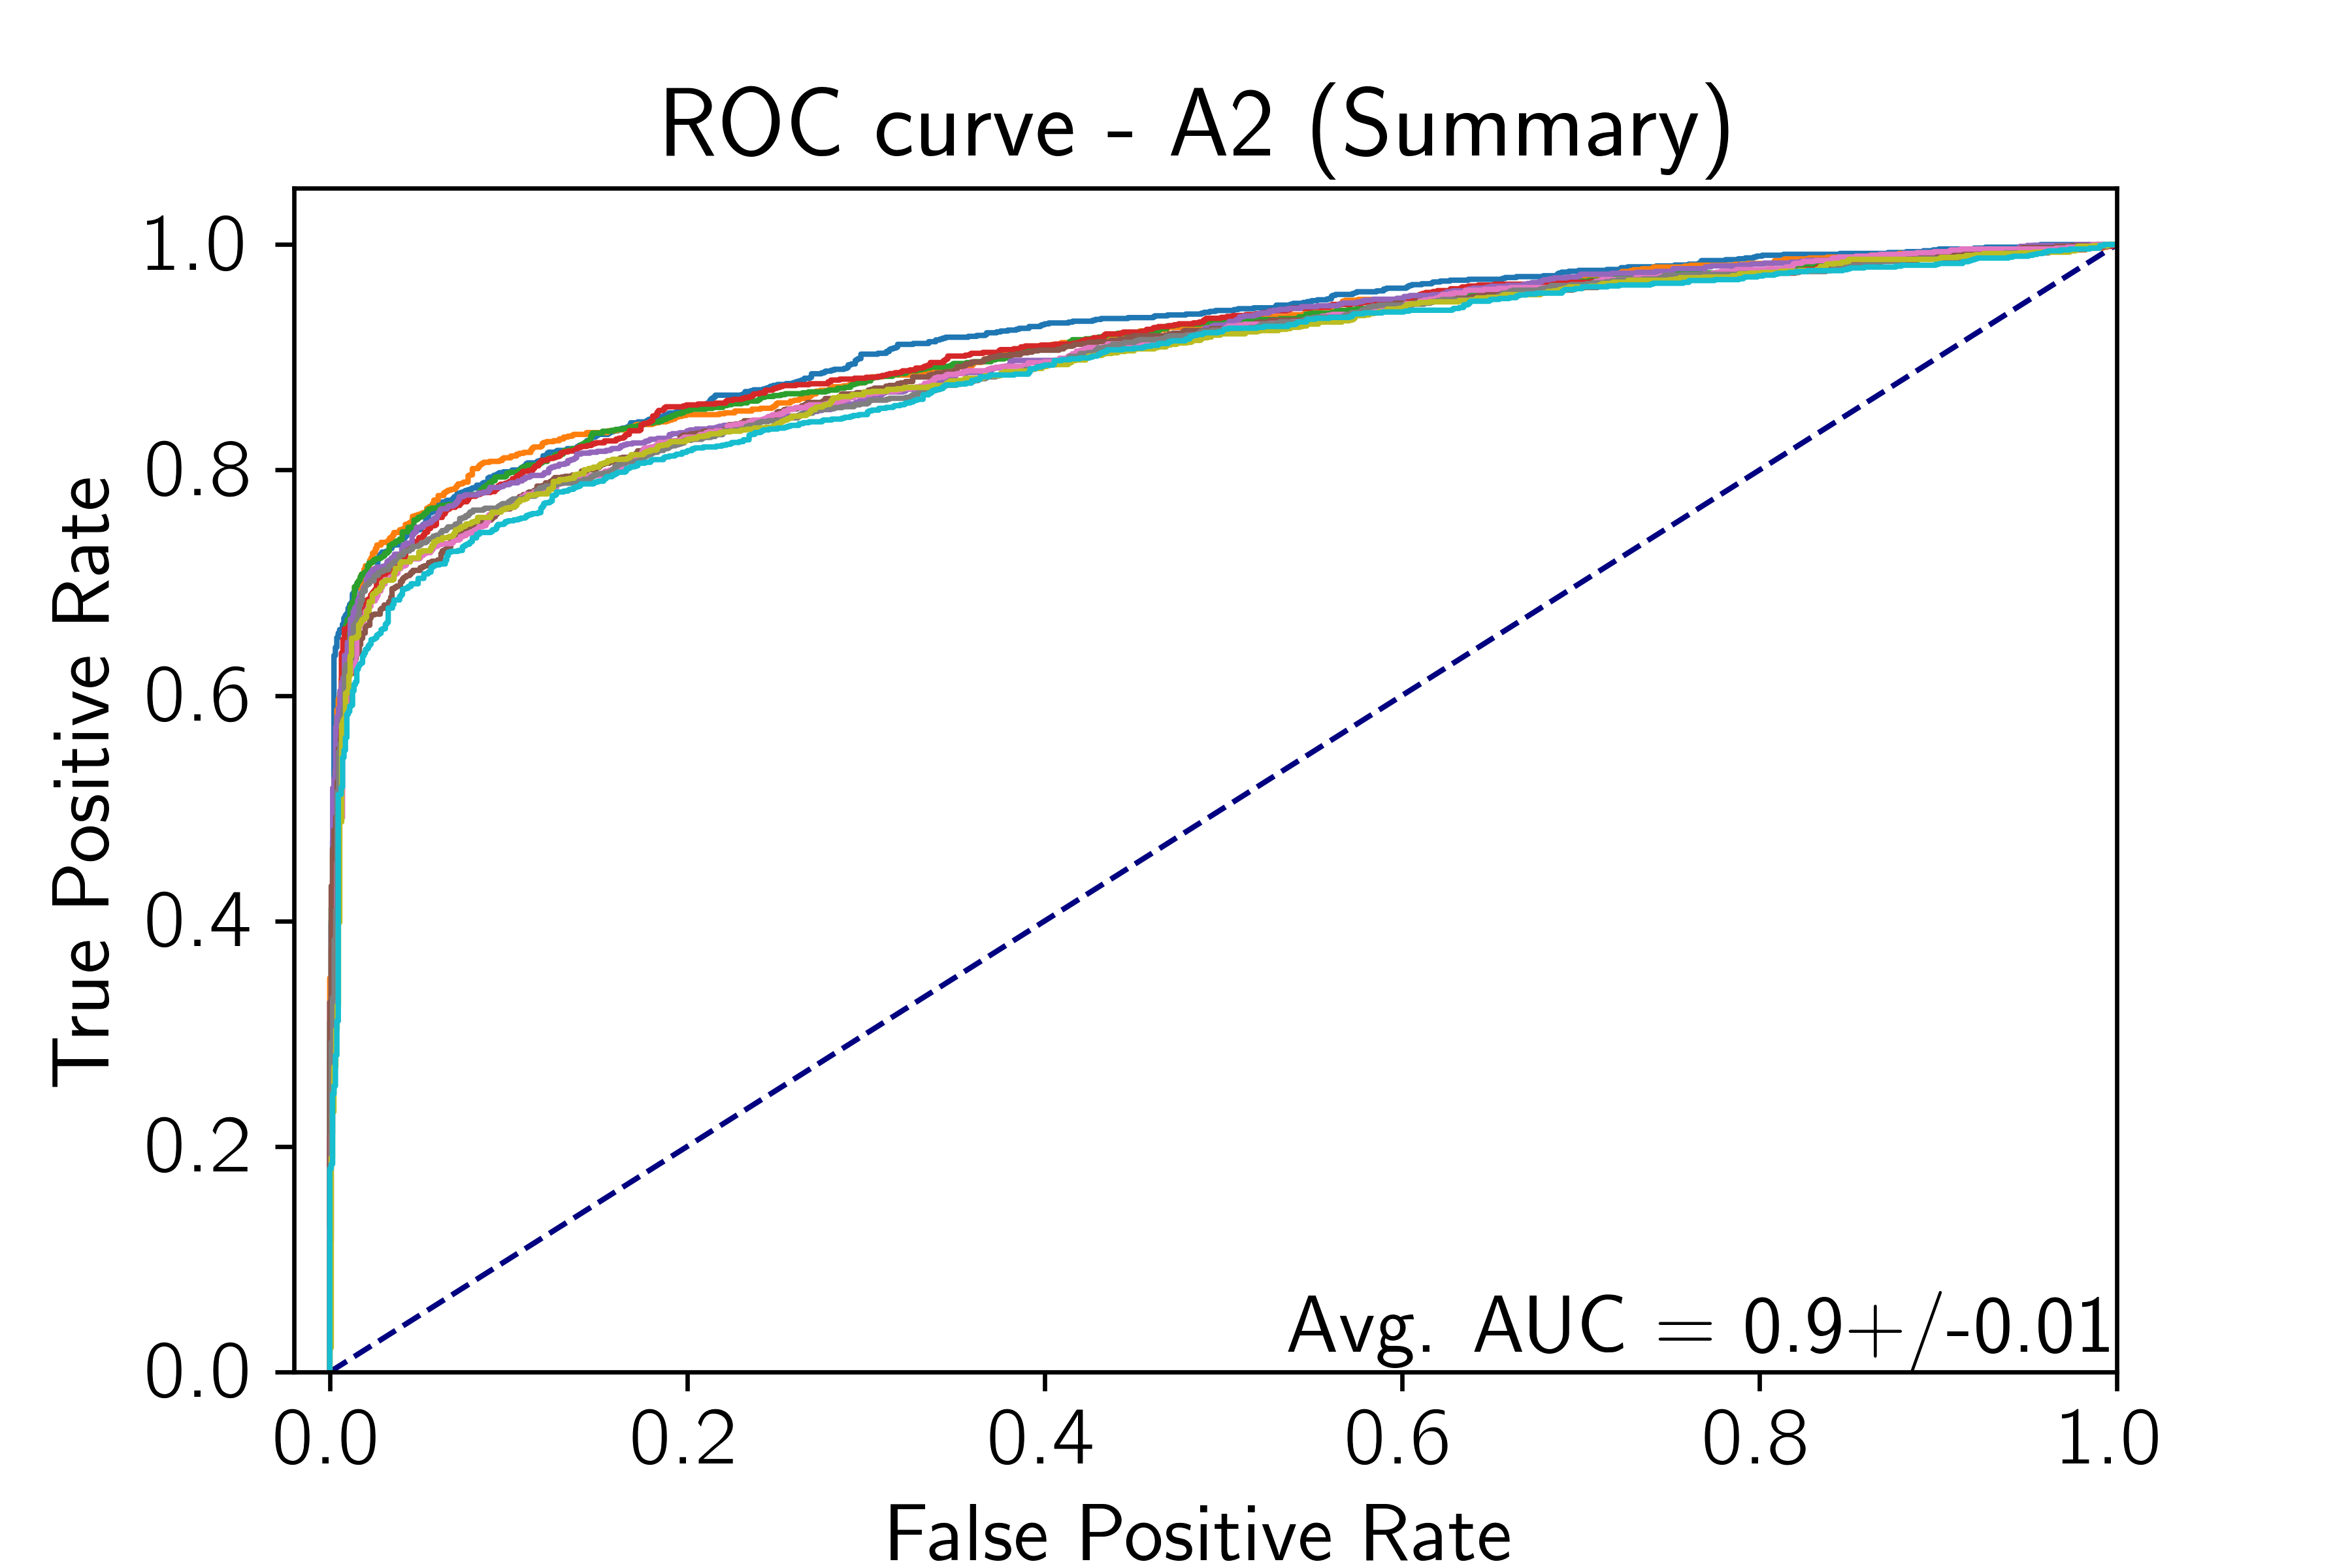
\includegraphics[width=0.48\columnwidth]{ML_Metric/ROCA2_SUMMARY}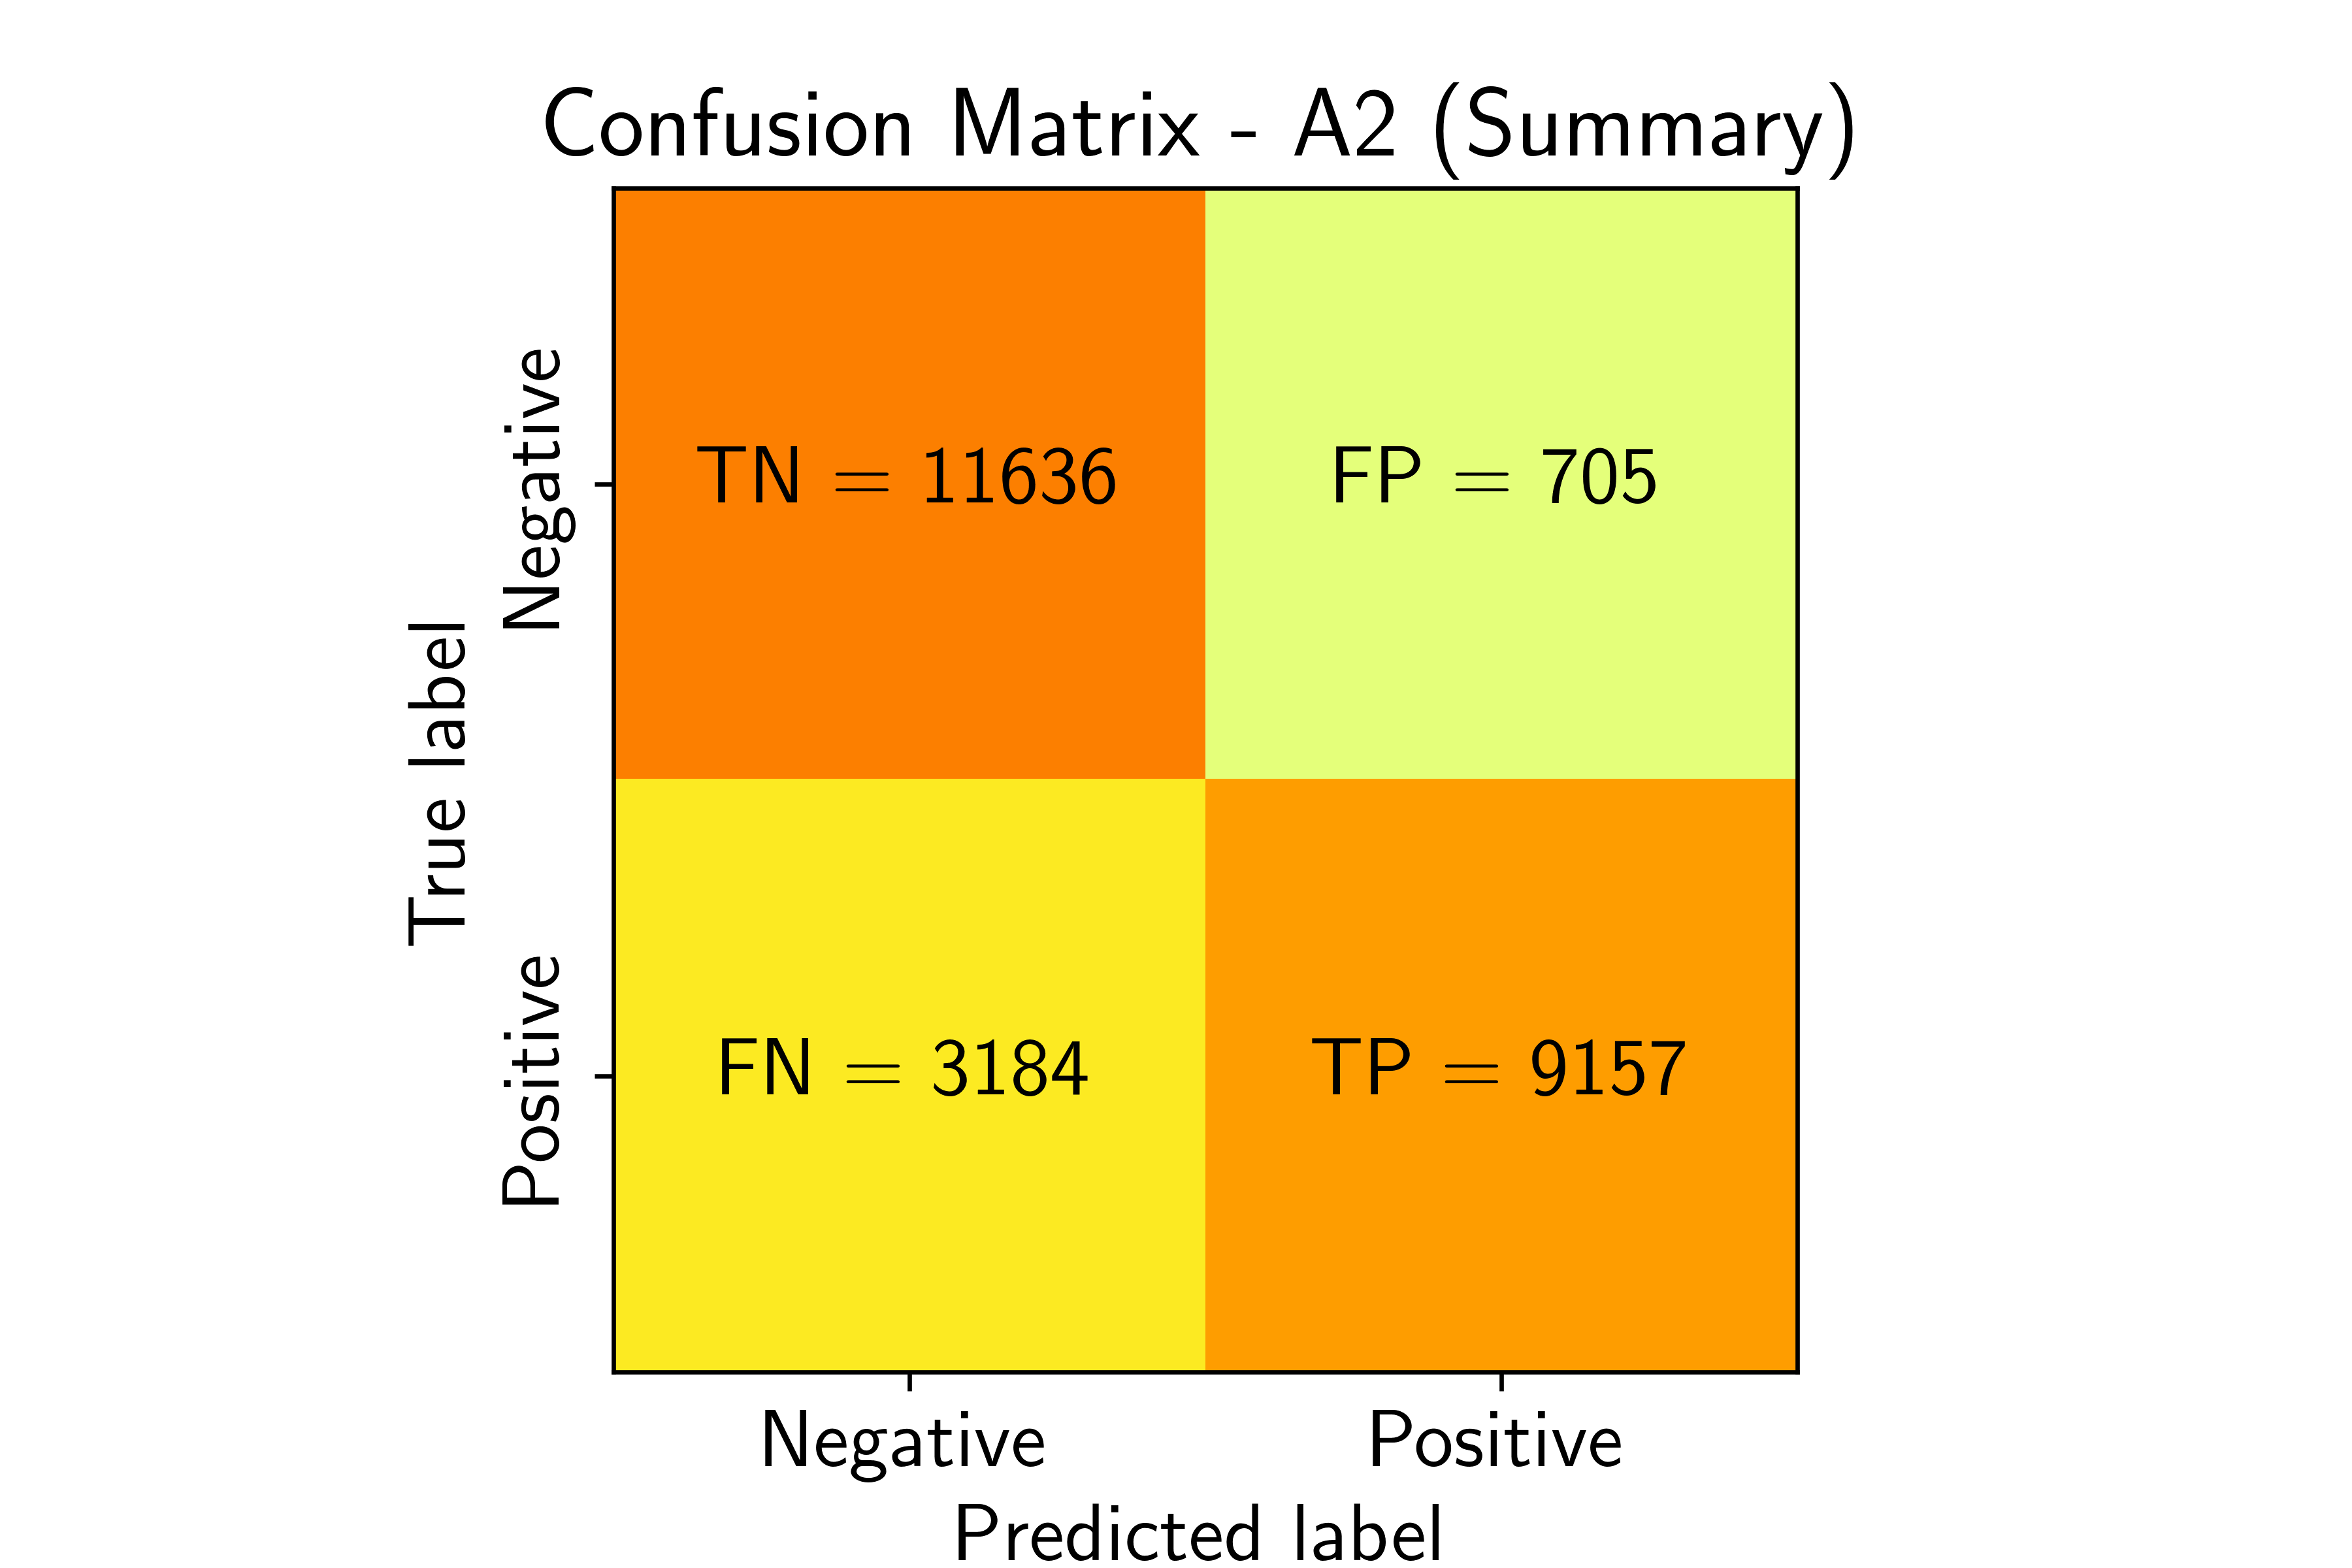
\includegraphics[width=0.48\columnwidth]{ML_Metric/CMA2_SUMMARY}
\end{figure}

\begin{figure}[H]
\noindent \begin{centering}
\caption{\label{F3}Results fir \texttt{Node2Vec} model with A3 feature}
\par\end{centering}
\noindent \raggedleft{}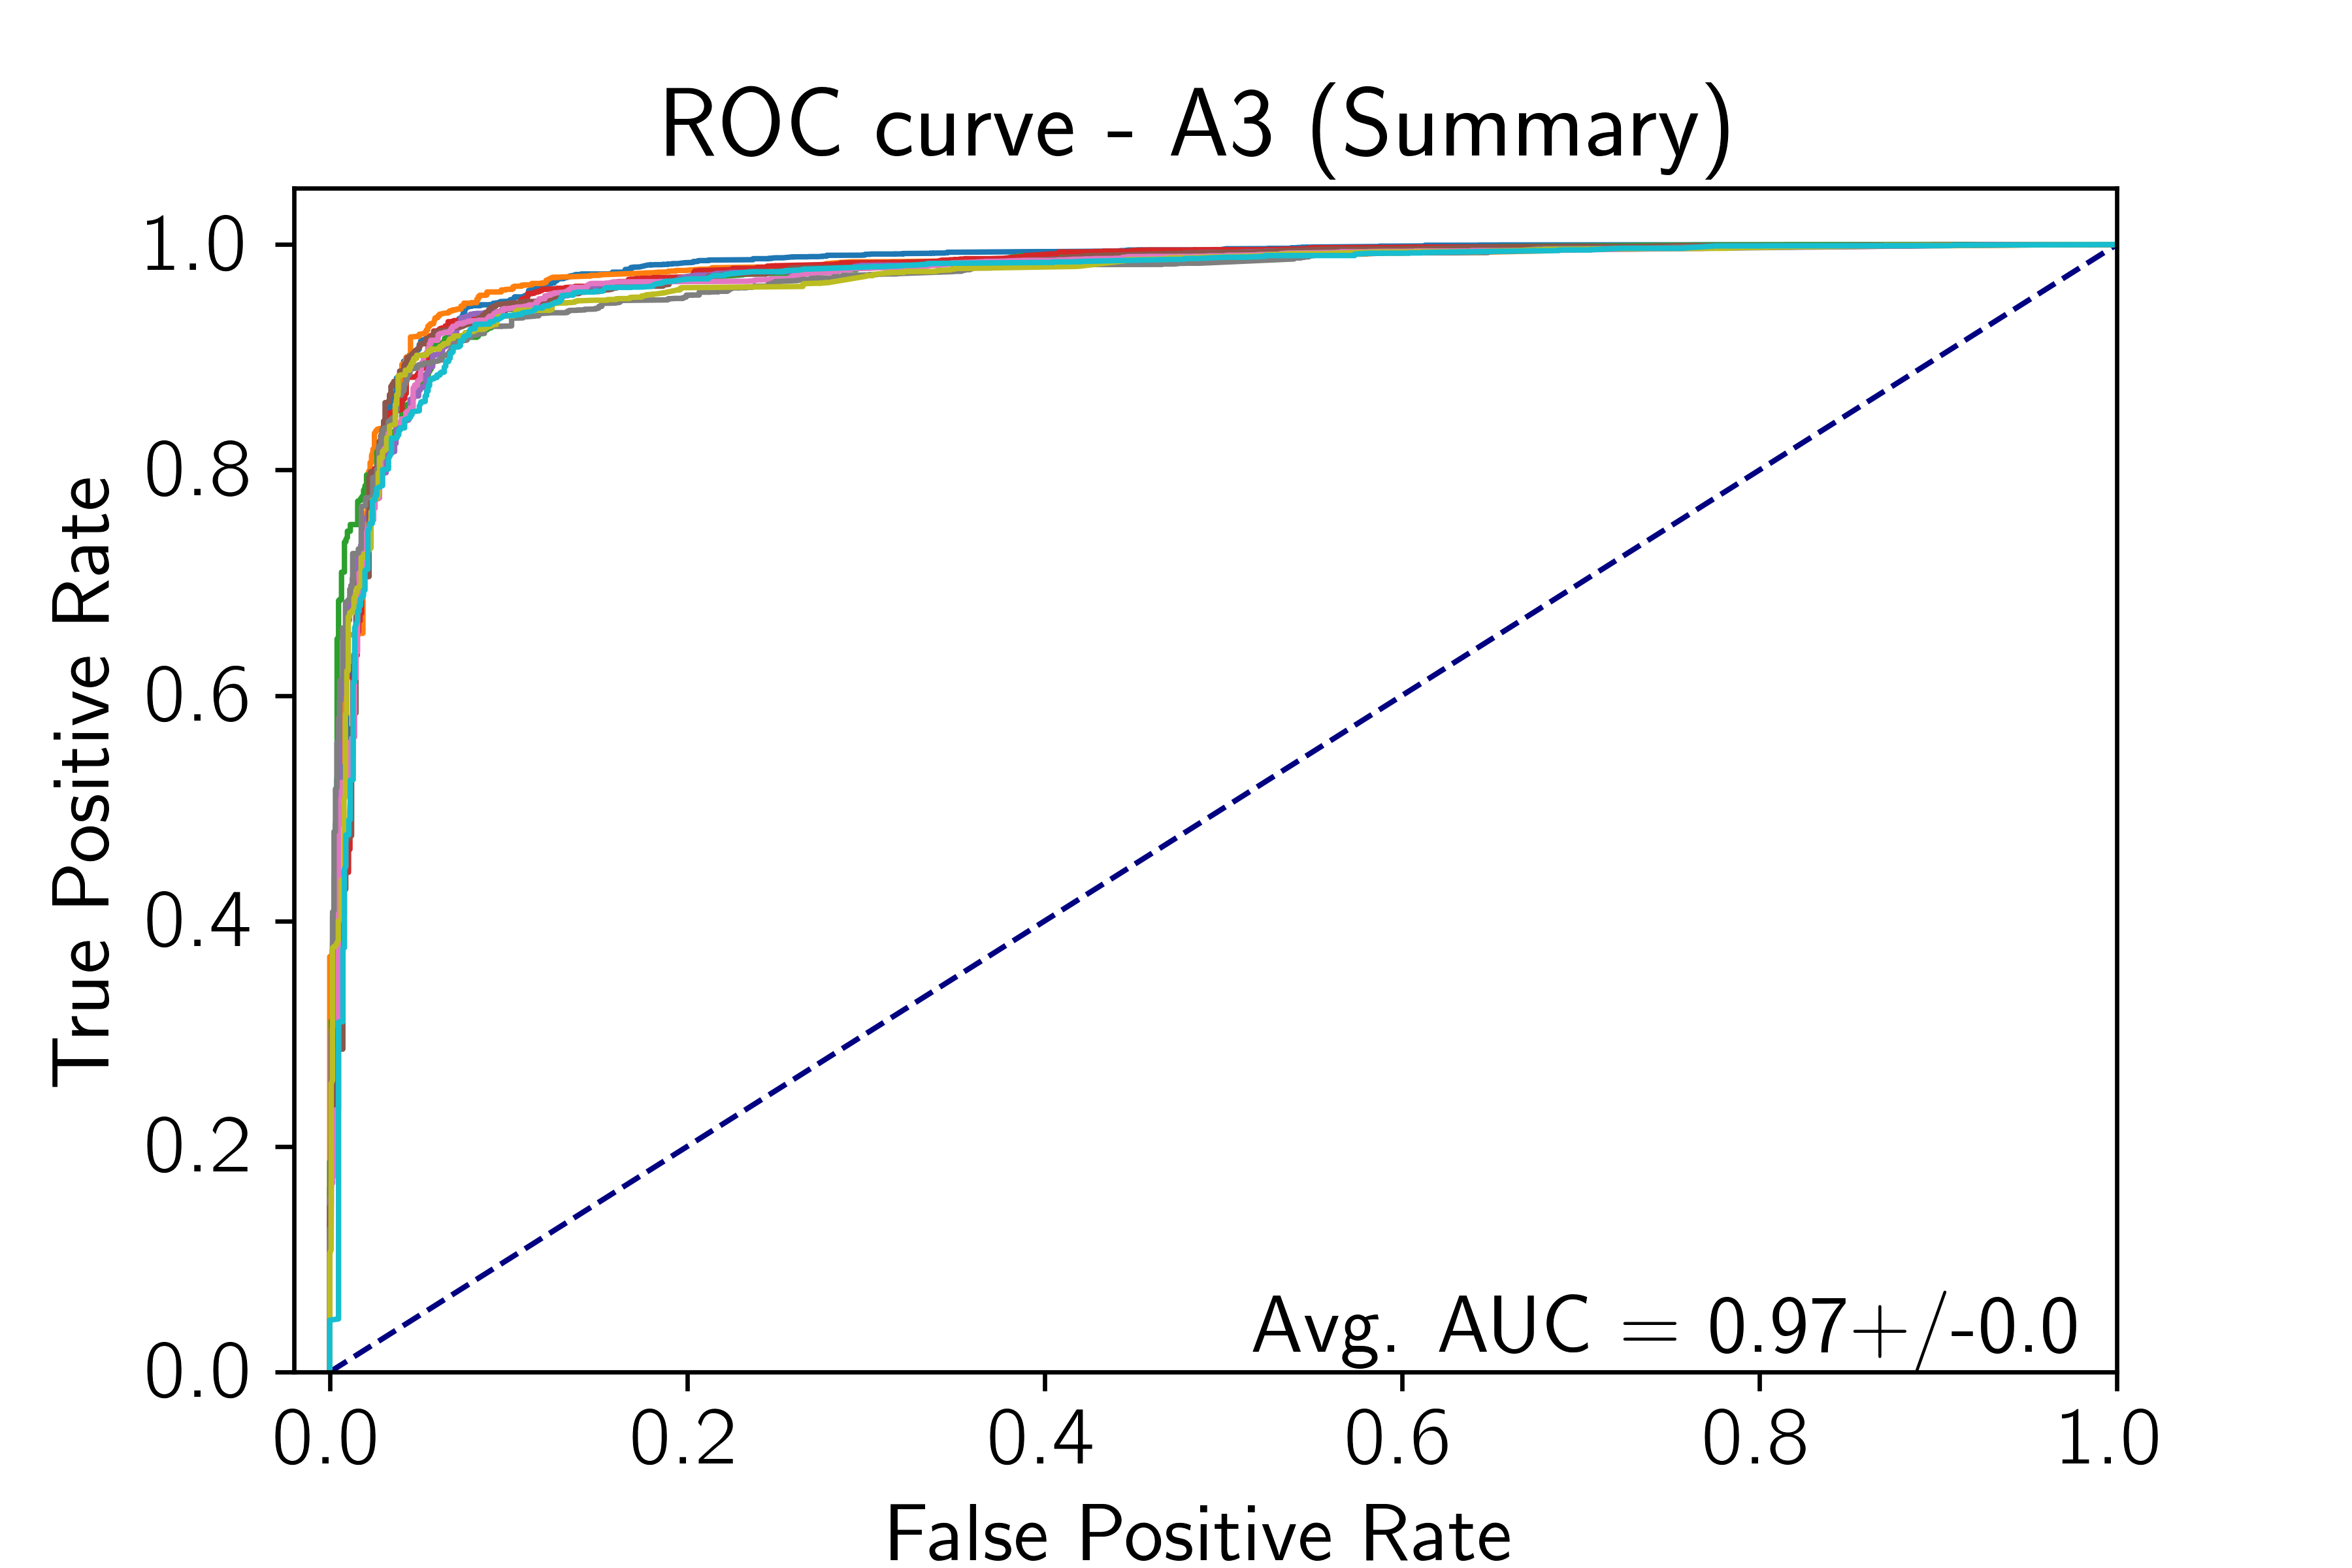
\includegraphics[width=0.48\columnwidth]{ML_Metric/ROCA3_SUMMARY}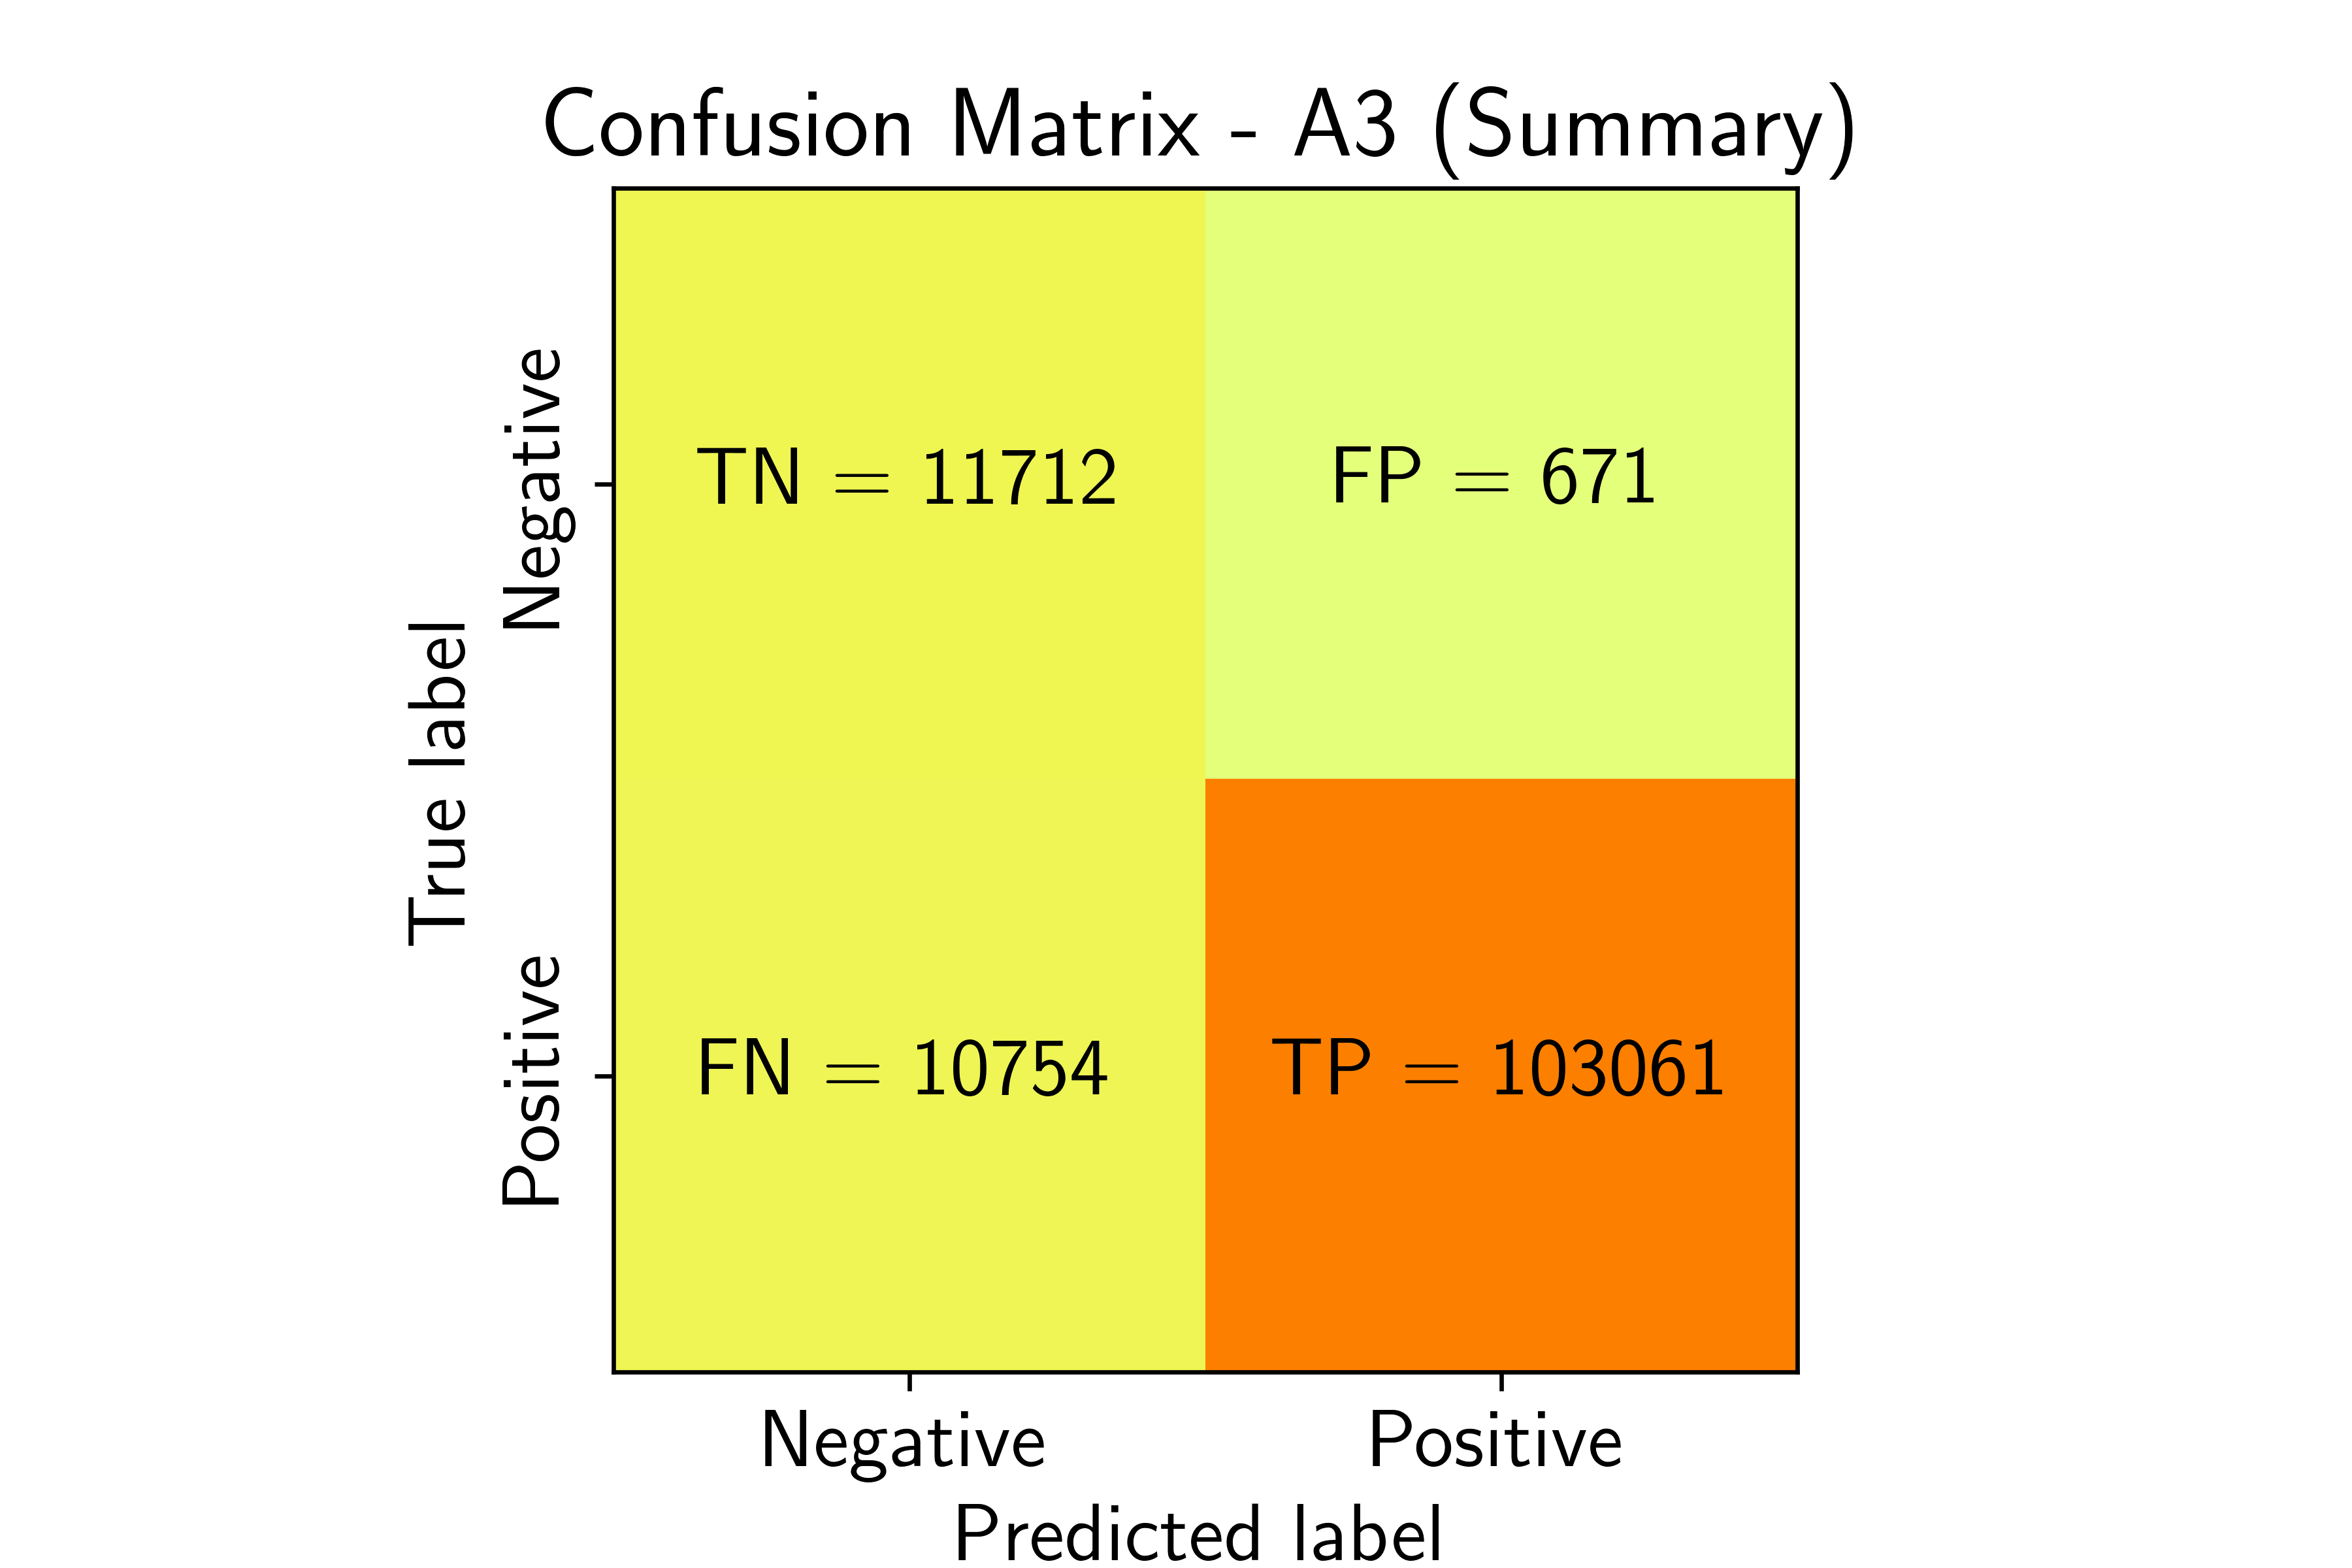
\includegraphics[width=0.48\columnwidth]{ML_Metric/CMA3_SUMMARY}
\end{figure}

\begin{figure}[H]
\noindent \begin{centering}
\caption{\label{F4}Results for \texttt{Node2Vec} model with L3 feature}
\par\end{centering}
\noindent \raggedleft{}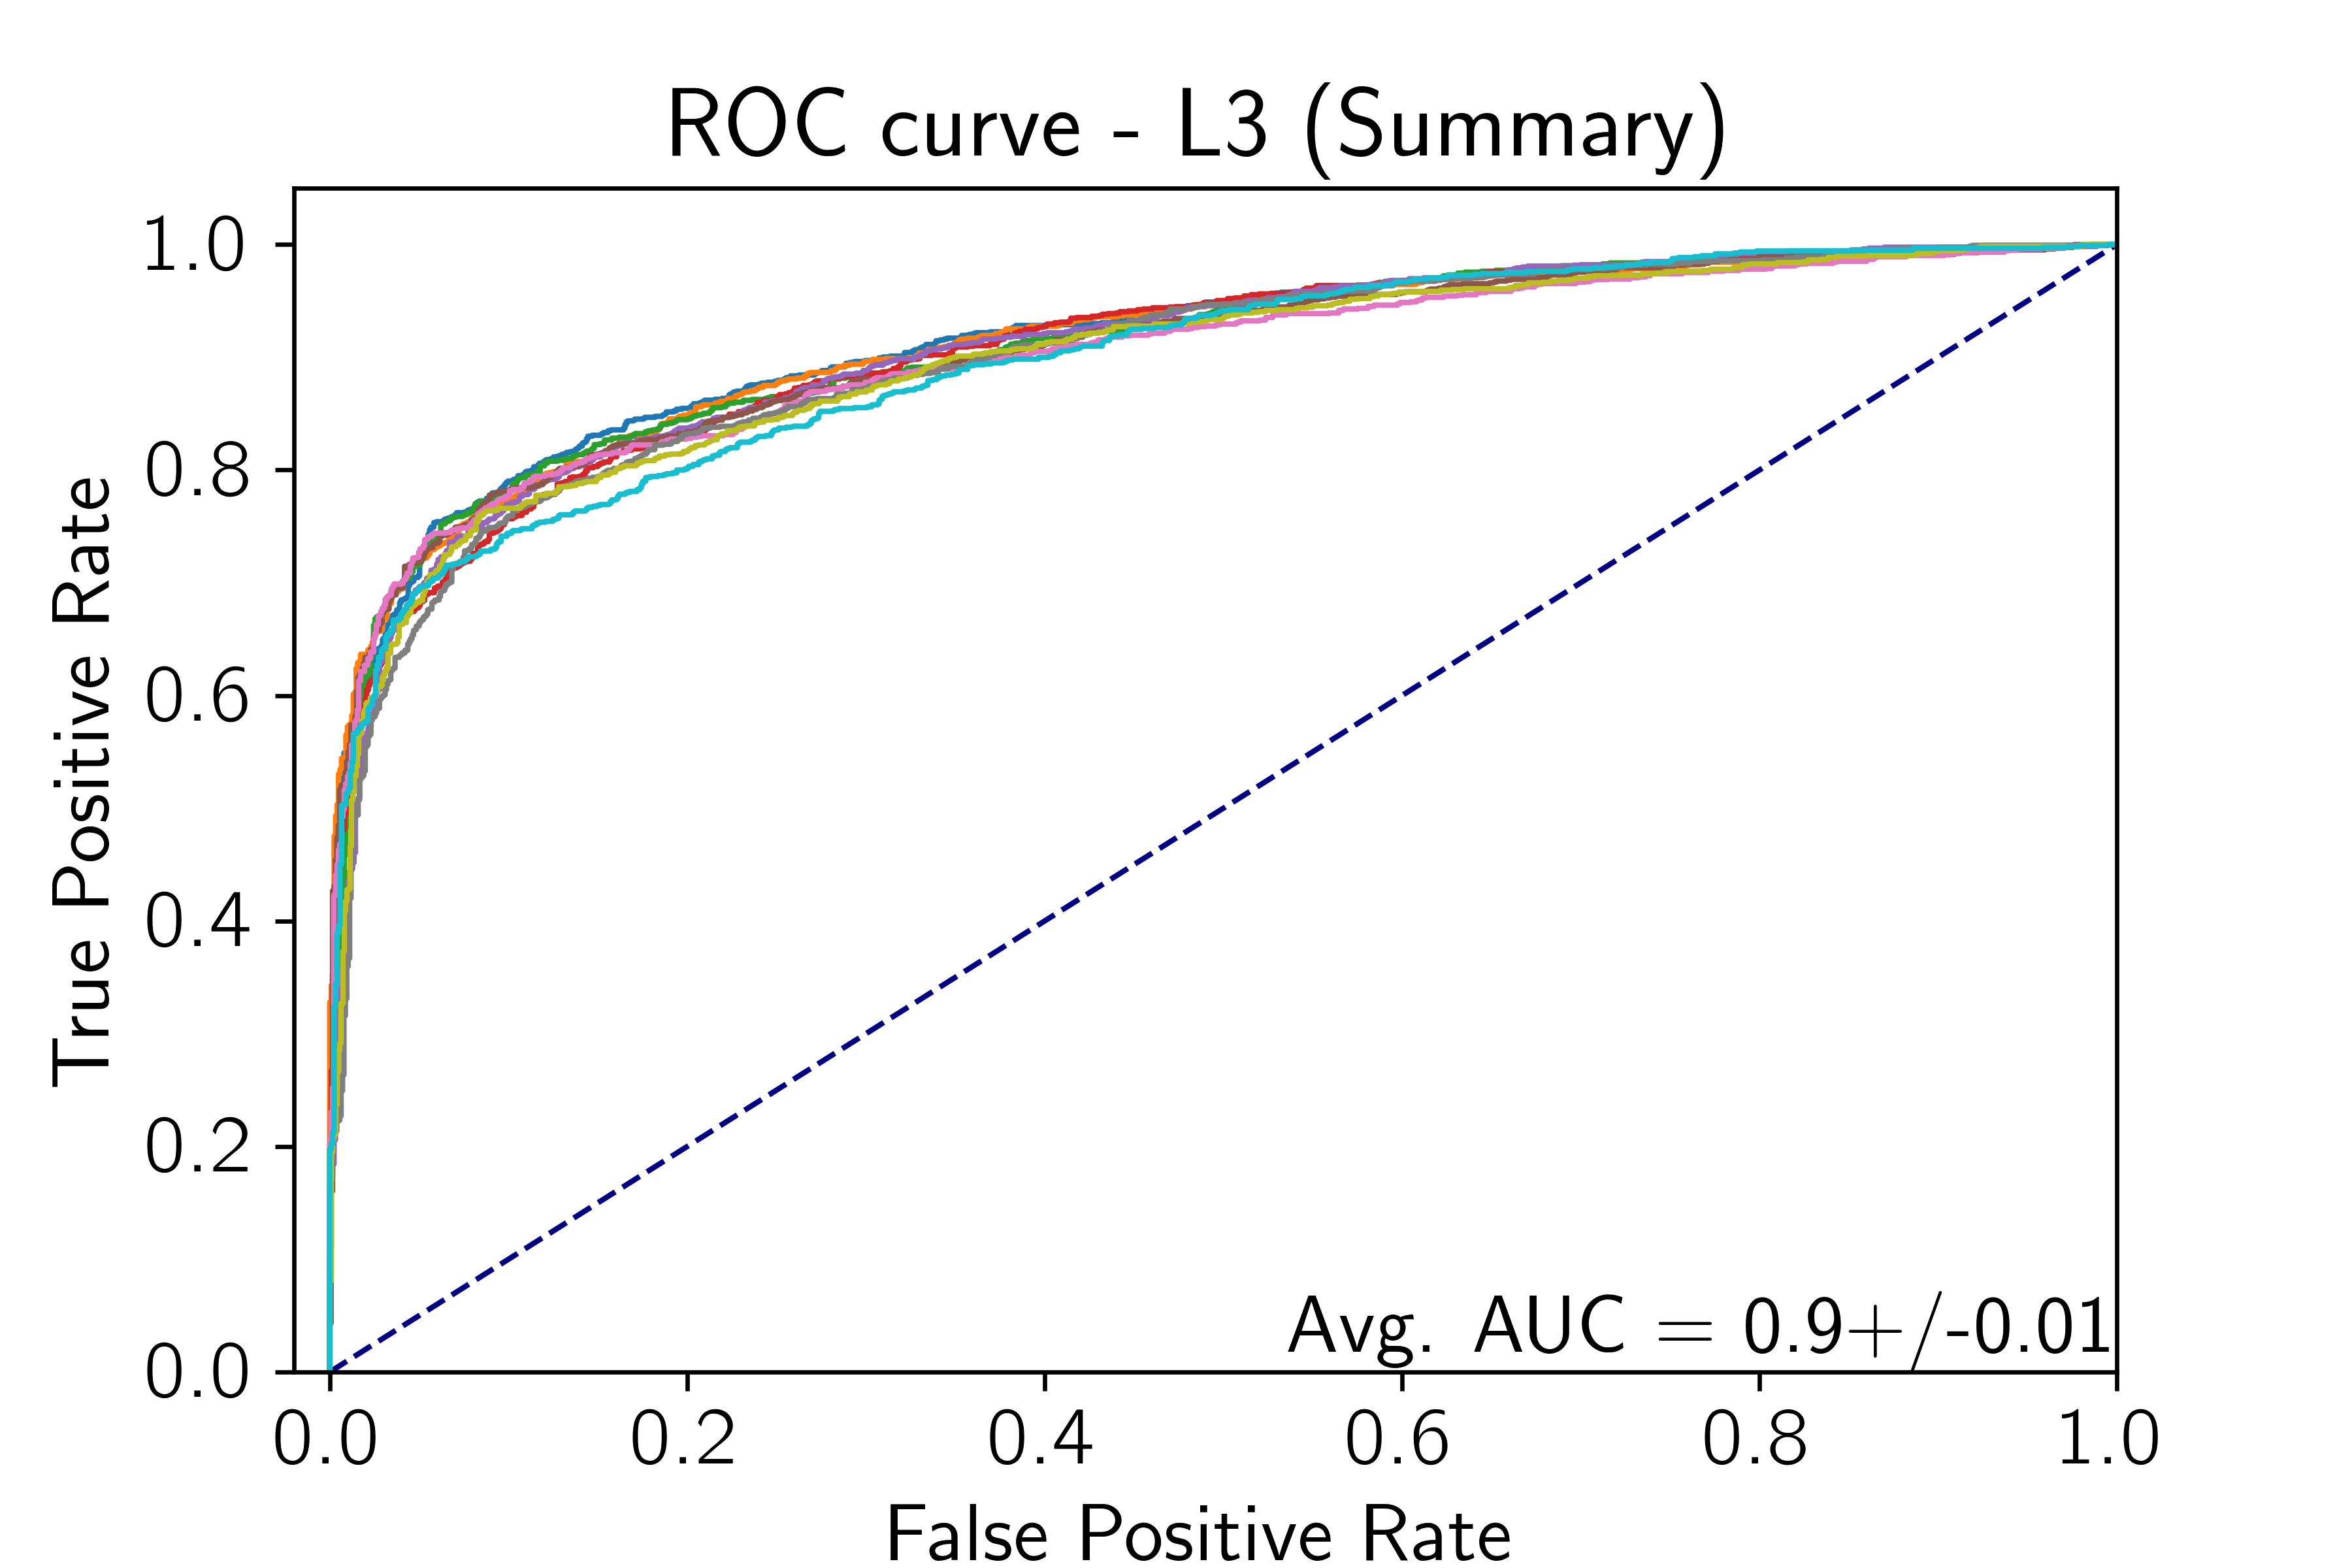
\includegraphics[width=0.48\columnwidth]{ML_Metric/ROCL3_SUMMARY}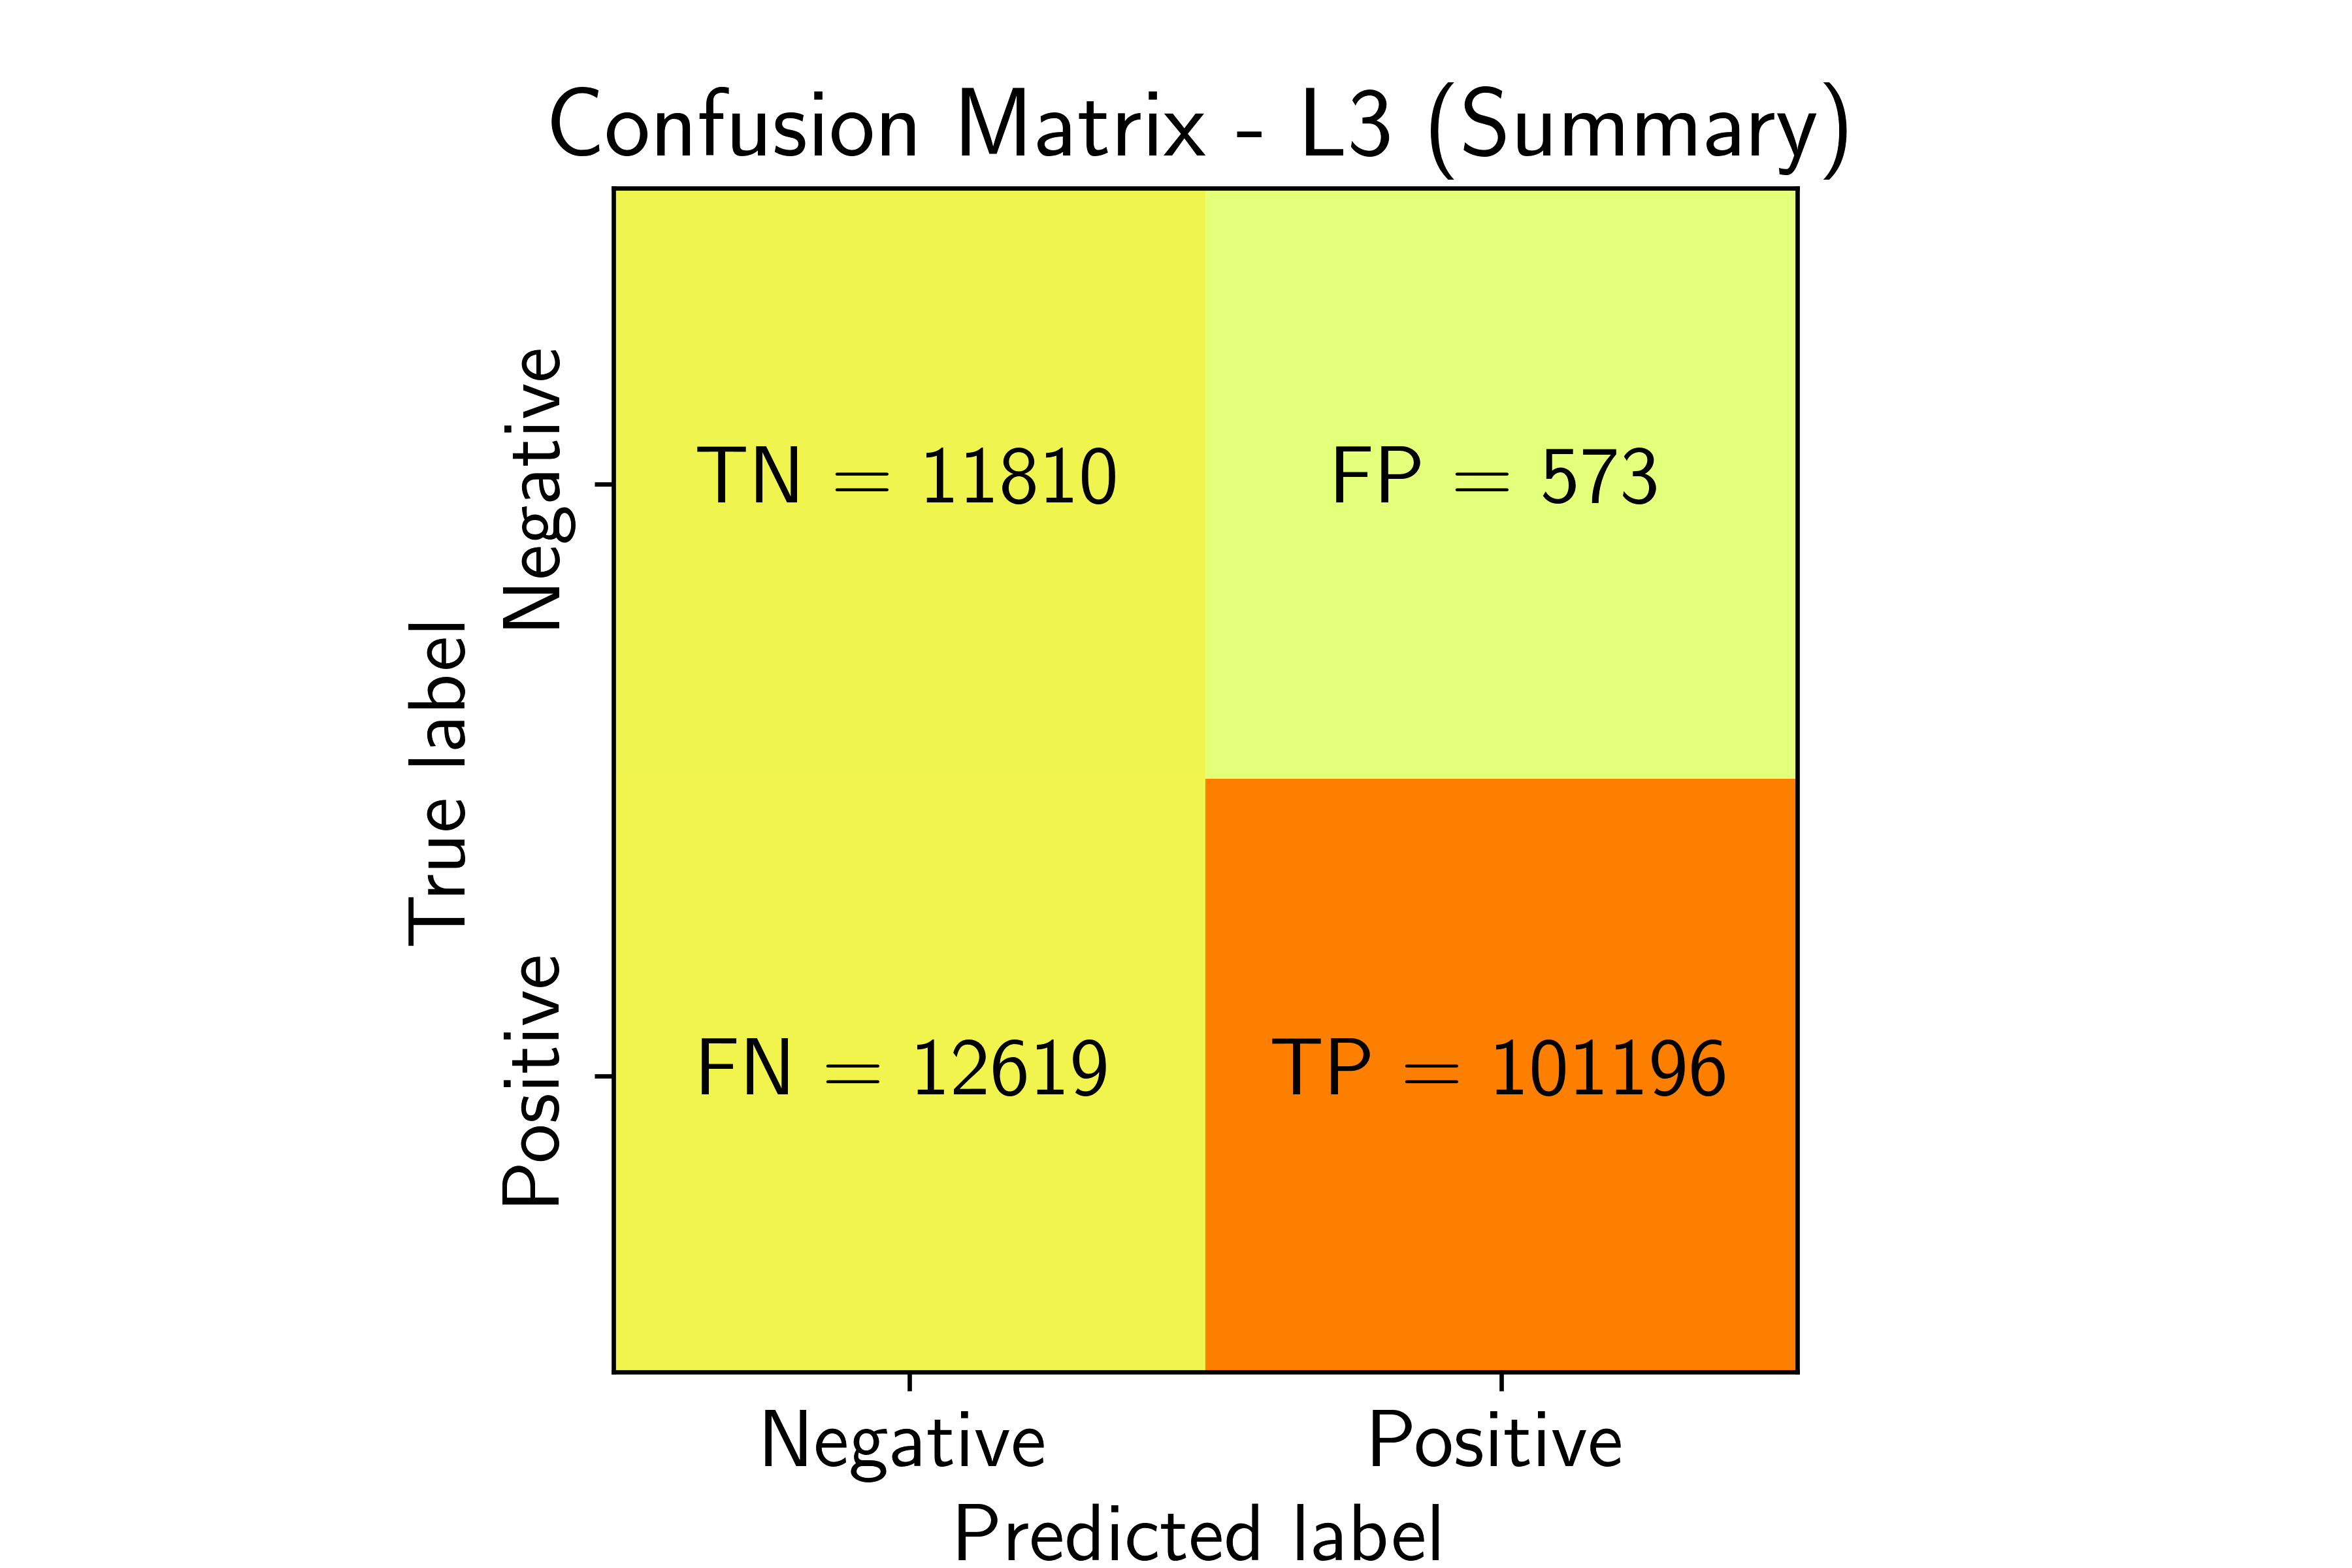
\includegraphics[width=0.48\columnwidth]{ML_Metric/CML3_SUMMARY}
\end{figure}

The precision when using the count of paths of length 3 (A3) is $0.86$
while the recall is $0.77$. It is interesting to observe that precision
decreased $7.5\%$ when compared to the previous case, but recall
increased $3.6\%$. A similar situation is obtained for the model
with the normalized score (L3), whose precision decreased to $0.89$
($-3.8\%$) and recall increased to $0.76$ ($+2.6\%$). It can
be seen also that the ROC curve rapidly achieves higher values of
true positive rate in the A2-featured model when compared to the other
models.

Finally, an relevant evaluation on the models that include a handcrafted
feature is necessary: How important is the appended feature for the
model result? The answer can be observed by the feature importance
plots for CN, A3 and L3 in Figure \ref{F5-importance}. Each plot
resembles the number of times that each feature creates a bifurcation
in the underlying decision trees that \texttt{XGBoost} uses. The more
bifurcations, the higher the importance a feature has on the model
itself. All models have the appended feature as the most important
by a large margin.

\begin{figure}[H]
\noindent \begin{centering}
\caption{\label{F5-importance}Importance for \texttt{Node2Vec} models: with
L3 feature}
\par\end{centering}
\noindent \begin{raggedleft}
\includegraphics[width=0.8\columnwidth]{ML_Metric/Imp\lyxdot A2\lyxdot 1}
\par\end{raggedleft}
\noindent \begin{raggedleft}
\includegraphics[width=0.8\columnwidth]{ML_Metric/Imp\lyxdot A3\lyxdot 1}
\par\end{raggedleft}
\noindent \raggedleft{}\includegraphics[width=0.8\columnwidth]{ML_Metric/Imp\lyxdot L3\lyxdot 1}
\end{figure}


\subsection{Human Interactome}

(PENDING FROM HERE)

\begin{figure}[h]
\caption{Methods Comparison for \emph{HI-II-14}}

\noindent \centering{}\includegraphics[width=1\columnwidth]{hi-ii-14\lyxdot txt}
\end{figure}

\begin{figure}[h]
\caption{Methods Comparison for \emph{HI-TESTED}}

\noindent \centering{}\includegraphics[width=1\columnwidth]{hi-tested\lyxdot txt}
\end{figure}

As it can be inferred from the plots, L3-based predictions outperform
their $A{{}^2}$ counterparts. Results also show that L3-score and
$A^{3}$predictions follow a very similar trend. 

\section{Conclusions}

Taking into account the different results validated in this paper,
one can conclude that length-3 path methodologies 
% what are the L3 methodologies, in the introduction only one is mentioned
might work better
on protein-protein interactions than its traditional length-2 (TCP
based) counterparts. On the other hand, it can be seen that degree-normalization
has little effect on the predictions, i.e., non-normalized $A{{}^3}$
matrix predictions are still a good methodology for edge prediction
on PPI networks.

Previous result comes as no surprise when the biological basis of
protein interactions is considered: It is necessary that protein A
and protein B have complementary structures in order to interact,
and when classical paths of length 2 are used, the predicted protein
interactions usually have the same structures, and not complementary
ones.

\begin{comment}
JF: please update the conclusions - WSD does not seem relevant

NL: Done
\end{comment}

\bibliographystyle{plain}
\bibliography{refs}

\end{document}
